\documentclass[t,% Place text of slides at the (vertical) top of the slides
brazilian,% Brazilian Portuguese, FTW!
11pt,% Standard font size
aspectratio=169,% Aspect ratio 16:9 (widescreen)
table% xcolor option
]{beamer}

\setbeamercolor{footnote mark}{fg=red}

\usetheme{Boadilla}
\setbeamertemplate{navigation symbols}{}
\setbeamertemplate{frametitle continuation}{}
\setbeamertemplate{page number in head/foot}[framenumber]
\setbeamertemplate{enumerate items}[default]
\setbeamertemplate{itemize items}[circle]
\setbeamercovered{transparent}
\setbeamerfont{frametitle}{size=\normalsize}

\usepackage{babel}
\usepackage[utf8]{inputenc}
\usepackage[T1]{fontenc}
\usepackage{lmodern}

\usepackage{graphicx}
\setkeys{Gin}{keepaspectratio}

\usepackage{amssymb,amsfonts,amsmath}
\usepackage{mathtools}

\usepackage{siunitx}
\sisetup{locale = FR}

\usepackage{tikz}
\usetikzlibrary{calc}

\usepackage{pgffor}
\usepackage{etoolbox}

% \usepackage{colortbl}

\usepackage{tcolorbox}

\usepackage{pgfplots}
\pgfplotsset{compat=1.18}

\newcommand{\esima}{\textordfeminine }
\newcommand{\esimo}{\textordmasculine }

\newcommand{\vboxcorr}[2]{%
    \resizebox{!}{\totalheight-#1}{%
        #2%
        }%
}
\newcommand{\hboxcorr}[2]{%
    \resizebox{\width-#1}{!}{#2}%
}

\DeclareMathOperator{\arctg}{arctg}
\DeclareMathOperator{\sen}{sen}
\DeclareMathOperator{\arcsen}{arc sen}

\def\Disciplina{Fenômenos de Transporte}
\def\Professor{Rodrigo de Farias Gomes}
\def\Periodo{Período 2025.1}

\title{\Disciplina}
\author{\Professor}
\date{\Periodo}

\begin{document}

\begin{frame}
    \titlepage
\end{frame}

\begin{frame}{Informações gerais}
    \begin{itemize}
        \item Nome: {\fontfamily{augie}\selectfont Rodrigo de Farias Gomes}
        \item Telefone (somente mensagens): (92) 9 9405-1724
        \item E-mail: shpnft@gmail.com
        \item Sala: 201b, Bloco E (2\esimo{} pavimento)
    \end{itemize}
\end{frame}

\begin{frame}{Avaliação}
    \begin{itemize}
        \item A avaliação será na forma de 3 notas: \(N_1\), \(N_2\) e \(N_3\)
        \item A média dos exercícios escolares (\(ME\)) será dada por
            \[
                ME=\frac{N_1+N_2+N_3}{3}
            \]
        \item Se \(MEE \geq 8,0\), então a média final (\(MF\)) será igual à \(MEE\)
        \item Se \(MEE < 8,0\), então
            \[
                MF=\frac{2\times MEE+PF}{3}
            \]
            onde PF é a nota da \textbf{prova final}
        \item A prova final abordará o mesmo \textit{conteúdo} da última prova realizada
        \item Se \(MF \geq 5,0\) e a frequência em sala for maior que 75\%, o aluno está aprovado
    \end{itemize}
\end{frame}


\begin{frame}<1>[label=ementa]{Ementa de \Disciplina}
    \begin{itemize}
        \item Conceitos e definições fundamentais
        \item Conceitos de Fenômenos de Transporte e
            Analogia entre os Processos Difusivos Unidimensionais de
            Transferência de Movimento Linear, de Calor e de Massa
        \item Fundamentos da Estática dos Fluidos
        \item Descrição e Classificação de Escoamentos
        \item Introdução à Análise de Escoamentos na Formulação de Volume de Controle
        \item Introdução à Análise Diferencial de Escoamentos
        \item Introdução à Transferência de Calor
        \item Introdução à Condução Unidimensional de Calor em Regime Permanente
        \item Introdução à Condução de Calor em Regime Transiente
        \item Introdução à Transferência de Massa
    \end{itemize}
\end{frame}

\begin{frame}{Livro}
    \centering
    \vboxcorr{27pt}{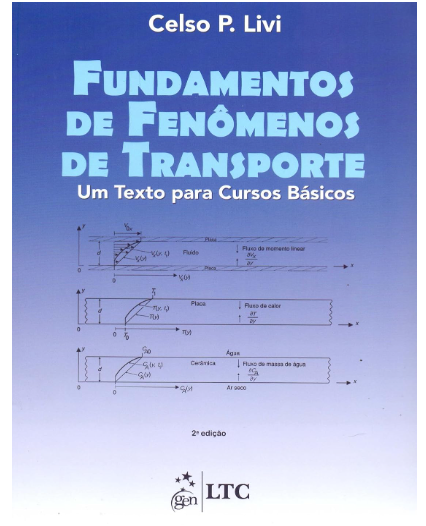
\includegraphics[height=\textheight]{images/Captura de tela de 2025-03-18 15-21-27.png}}
\end{frame}

\begin{frame}{Capítulos do Livro}
    \centering
    \vboxcorr{27pt}{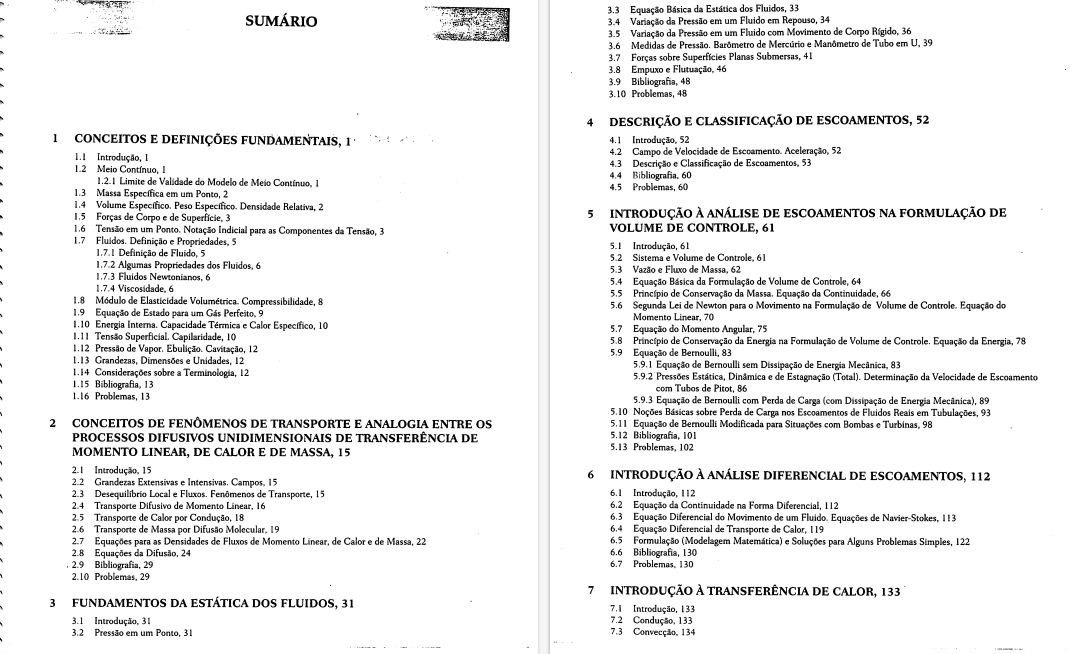
\includegraphics[height=\textheight]{images/Captura de tela de 2025-03-18 15-25-51.png}}
\end{frame}

\begin{frame}{Capítulos do Livro}
    \vboxcorr{27pt}{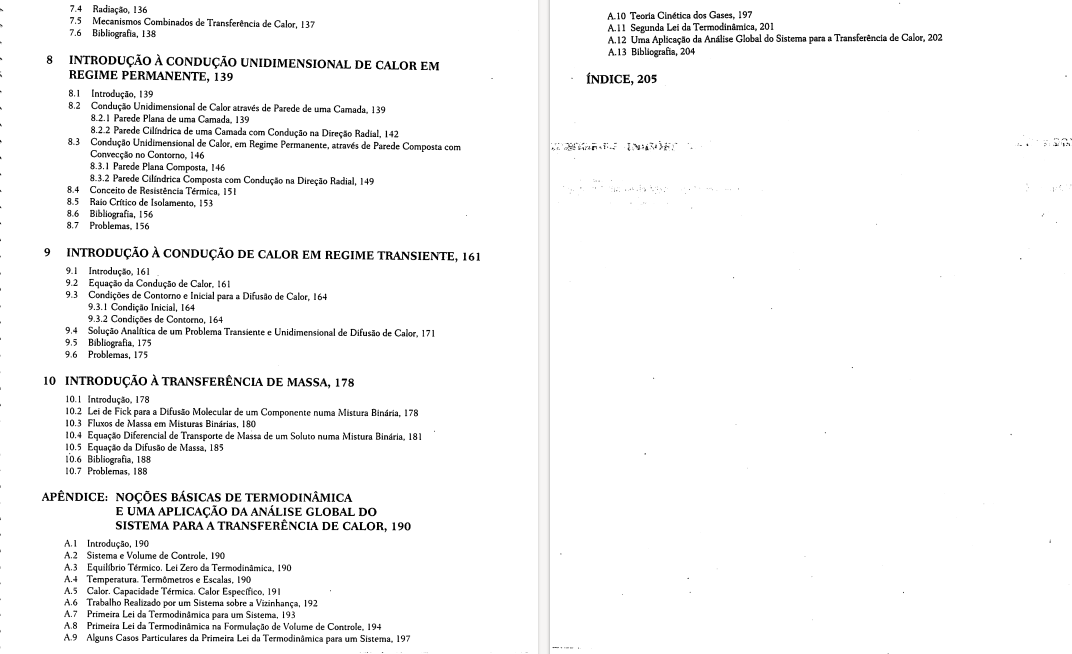
\includegraphics[height=\textheight]{images/Captura de tela de 2025-03-18 15-26-08.png}}
\end{frame}

\begin{frame}{Massa específica, volume específico e peso específico}
    \begin{itemize}
        \item Massa específica
            \[
                \rho = \lim_{\Delta V \to \delta V} \frac{\Delta m}{\Delta V} 
            \]
            onde:
            \begin{description}
                \item[\(\Delta m\)] é a massa contida no volume \(\Delta V\)
                \item[\(\delta V\)] é o menor volume onde seja válido o \textbf{modelo contínuo}
            \end{description}
        \item Volume específico
            \[
                v=\frac{1}{\rho}
            \]
        \item Peso específico
            \[
                \gamma = \rho g
            \]
    \end{itemize}
\end{frame}

\begin{frame}{Forças}
    \begin{itemize}
        \item Forças de corpo são aquelas que se manifestam através da interação com um campo e 
            atuam sem a necessidade de um contato entre as superfícies dos corpos.

            Exemplos: força peso, força elétrica, força magnética

            Forças de corpo são proporcionais ao volume dos corpos\footnote{Somente no caso de corpos uniformes}

        \item Forças de superfície são aquelas que atuam sobre um sistema através de contato com a fronteira do mesmo

            Exemplos: força de atrito, forças devido à \textit{pressão}

            Forças de superfície são proporcionais à área da superfície sobre a qual atuam
            \footnote{Somente no caso de corpos com superfícies uniformes}
    \end{itemize}
\end{frame}

\begin{frame}{Tensão e pressão}
    \begin{itemize}
        \item  A tensão é definida como a força por unidade de área aplicada a
            um corpo. Mas vimos em Física Geral II que pressão também é força
            por unidade de área. Qual a diferença?
        \item Pressão é uma grandeza \textbf{escalar} que só considera a componente \textit{normal} da força aplicada na superfície,
            enquanto a tensão é uma grandeza \textbf{tensorial} que considera todas as componentes
            \[
                \vec{\vec{T}}=
                \begin{bmatrix}
                    \sigma_{xx} & \tau_{xy} & \tau_{xz} \\ 
                    \tau_{yx} & \sigma_{yy} & \tau_{yz} \\
                    \tau_{zx} & \tau_{zy} & \sigma_{zz}
                \end{bmatrix}
            \]
            onde as \textbf{tensões normais} \(\sigma_{ii}\) são definidas como
            \[
                \sigma_{ii} = \lim_{\Delta A_i \to 0} \frac{\Delta F_i}{\Delta A_i}
            \]
            e as \textbf{tensões cisalhantes} (tangenciais) \(\tau_{ij}\) são definidas como
            \[
                \tau_{ij} = \lim_{\Delta A_i \to 0} \frac{\Delta F_j}{\Delta A_i}
            \]
    \end{itemize}
\end{frame}

\begin{frame}{Fluidos}
    \begin{itemize}
        \item A definição mais elementar de fluido diz: ''Fluido é uma
            substância que não tem uma forma própria, assume o formato do
            recipiente''
        \item Se o problema fundamental fosse apenas reconhecer os fluidos, a
            definição apresentada seria perfeitamente suficiente para essa
            finalidade
        \item Entretanto, vamos montar uma definição baseada na tensão de
            cisalhamento aplicada
        \item Seja um sólido preso entre duas placas planas
            \begin{center}
                \hboxcorr{22pt}{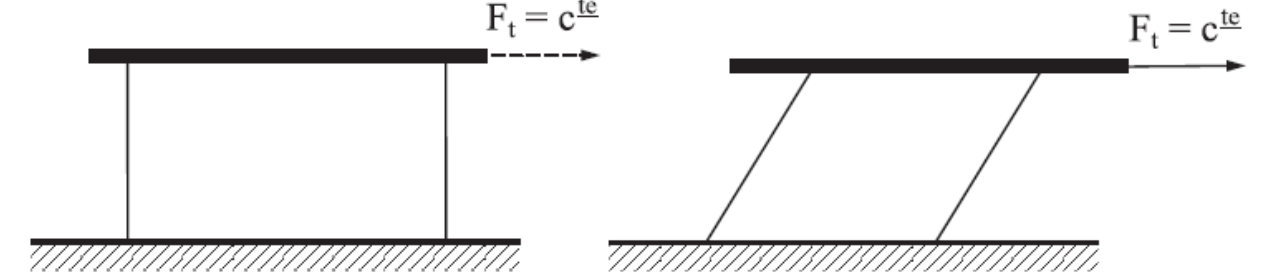
\includegraphics[width=\textwidth]{images/Captura de tela de 2025-03-25 15-37-33.png}}
            \end{center}
        \item Nota-se que o sólido se deforma até alcançar uma posição de
            equilíbrio estático
    \end{itemize}
\end{frame}

\begin{frame}
    \begin{itemize}
        \item Agora vamos colocando-se um fluido entre as placas, ''assumindo''
            que seja possível visualizar um certo volume \(ABCD\) do fluido
            \begin{center}
                \hboxcorr{22pt}{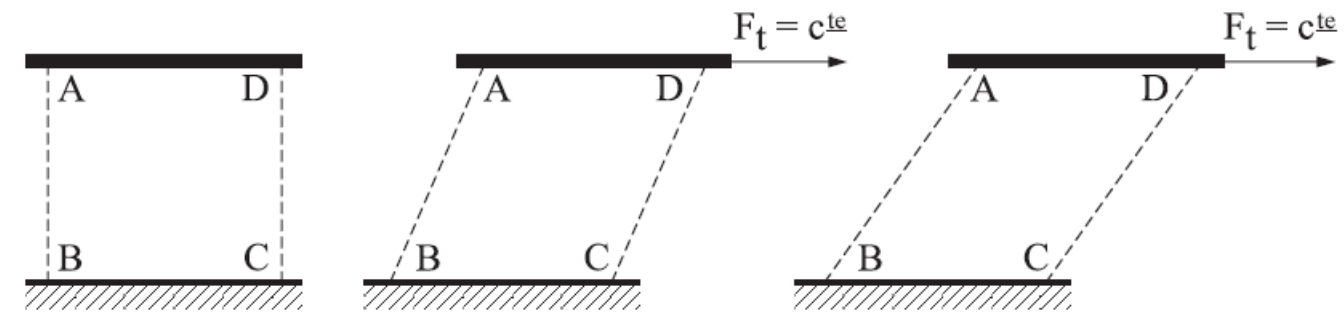
\includegraphics[width=\textwidth]{images/Captura de tela de 2025-03-25 15-42-52.png}}
            \end{center}
        \item \textbf{Princípio da Aderência}: Os pontos de um fluido, em
            contato com uma superfície sólida, aderem aos pontos dela, com os
            quais estão em contato
        \item Ou seja,a velocidade do fluido em contato com a placa será a igual
            a velocidade da placa
        \item Ou seja, os fluidos se deformam continuamente
    \end{itemize}
\end{frame}

\begin{frame}
    \begin{itemize}
        \item Ou seja, ''Fluido é uma substância que se deforma continuamente sob a ação
            de uma tensão de cisalhamento, \textbf{por menor que ela seja}''
        \item Existindo tensão cisalhante o fluido entra em movimento, ou seja, ocorre \textbf{escoamento}
        \item Os fluidos se moldam ao formato dos recipientes que os contêm \footnote{Por quê?}
        \item Um fluido é incompressível se, ao ser submetido a uma tensão normal, não há
            variação volumétrica
        \item Para um fluido em repouso, a tensão é exclusivamente normal, sendo seu valor
            chamado de pressão estática \(p\) que, em um ponto, é igual em qualquer direção, ou seja
            \[
                \sigma_{xx}=
                \sigma_{yy}=
                \sigma_{zz}=-p
            \]
    \end{itemize}
    \pause
    \begin{block}{Problema 1.1 do livro texto}
        Os líquidos e gases são fluidos, mas apresentam características diferentes. Descreva as propriedades
        que diferenciam os gases dos líquidos
    \end{block}
\end{frame}

\begin{frame}{Viscosidade}
    \begin{itemize}
        \item Vamos analisar um pouco mais o caso do fluido entre placas
            \begin{center}
                \hboxcorr{22pt}{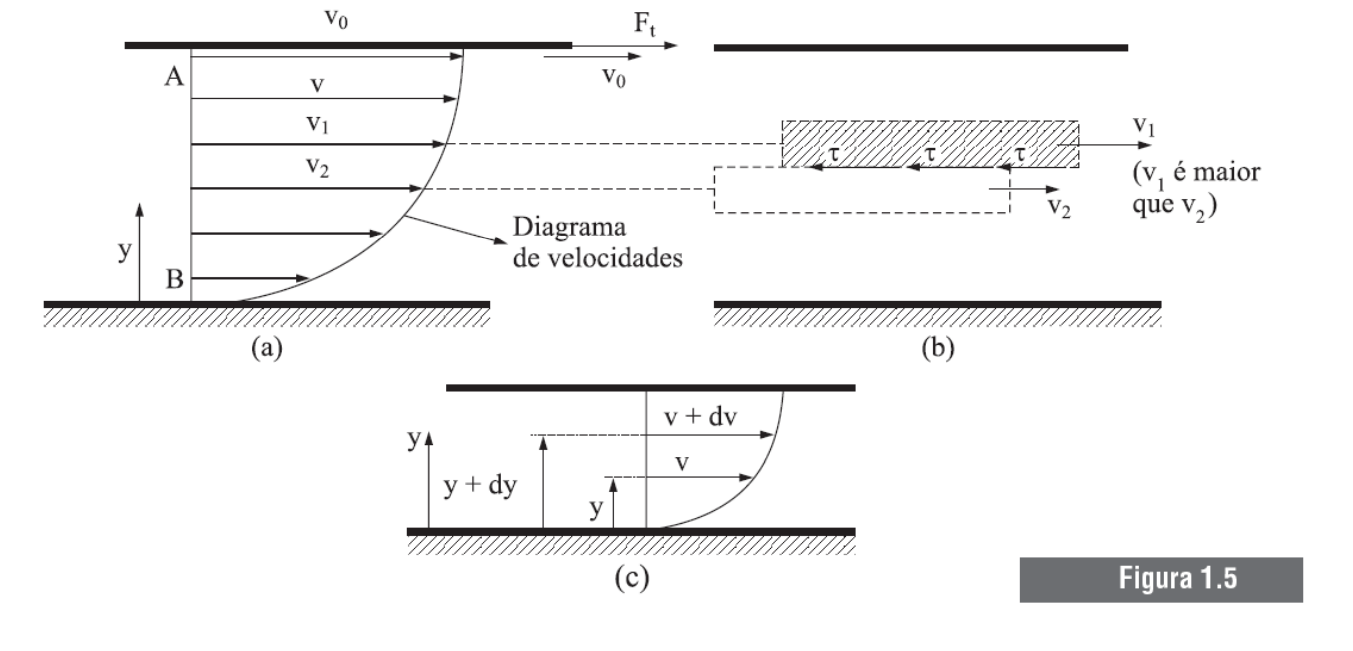
\includegraphics[width=\textwidth]{images/Captura de tela de 2025-03-25 16-11-12.png}}
            \end{center}
    \end{itemize}
\end{frame}

\begin{frame}
    \begin{itemize}
        \item Note que a diferença de velocidade \(v_1-v_2\) entre duas ''camadas'' do fluido pode ser
            explicada pela tensão de cisalhamento \(\tau\)
        \item Newton descobriu que em muitos fluidos \(\tau\) é proporcional a variação da velocidade com \(y\)
            \[
                \tau = \mu \frac{dv}{dy}
            \]
        \item Essa equação\footnote{No livro há um sinal negativo, mas vou
            omiti-lo por enquanto} é conhecida como \textbf{Lei de Newton para
            a Viscosidade} e \(\mu\) é a \textbf{viscosidade absoluta ou dinâmica}
        \item Os fluidos que obedecem a essa lei são ditos \textbf{fluidos newtonianos}, enquanto que
            os outros são chamados de \textbf{não newtonianos}
        \item Aqui só vamos tratar de fluidos newtonianos
    \end{itemize}
\end{frame}

\begin{frame}
    \begin{itemize}
        \item Podemos dizer que ''viscosidade é a propriedade que indica a maior ou menor dificuldade
            do fluido escoar''
        \item A viscosidade é causada fundamentalmente pela coesão intermolecular 
            e pela \textit{transferência de momento linear} através do fluido
        \item A viscosidade depende da temperatura, sendo que ela aumenta com a temperatura nos 
            gases e diminui com a temperatura nos líquidos\footnote{No livro texto há uma explicação para isso na página 8}
        \item No SI, a unidade da viscosidade absoluta é \(\si{Pa\cdot s}\)
        \item A viscosidade cinemática do fluido é dada por
            \[
                \nu = \frac{\mu}{\rho}
            \]
            onde \(\rho\) é a massa específica do fluido. A unidade de \(\nu\) no SI é 
            \(\si{m^2/s}\)
    \end{itemize}
\end{frame}

\begin{frame}{Problemas}
    \begin{itemize}
        \item [1.3] A figura 1.7 mostra o esquema de um escoamento de água entre duas placas
            planas horizontais de grandes dimensões e separadas por uma distância \(d\) pequena.
            A placa inferior permanece em repouso, enquanto a placa superior está em movimento com 
            velocidade \(V_x\) constante, de forma que resulta uma distribuição linear de velocidade
            de escoamento de água. Sendo a viscosidade da água \(\mu=\SI{1e-3}{Pa\cdot s}\), determine
            \begin{enumerate}[a)]
                \item o gradiente de velocidade de escoamento
                \item a tensão de cisalhamento na placa superior
            \end{enumerate}
    \end{itemize}
    \centering
    \vboxcorr{115pt}{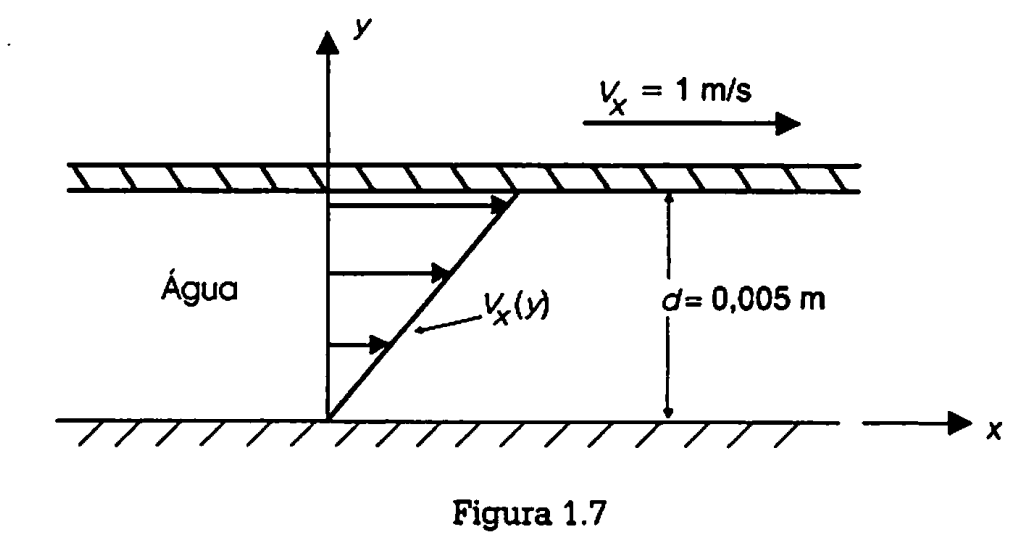
\includegraphics[height=\textheight]{images/Captura de tela de 2025-03-25 16-57-30.png}}
\end{frame}

\begin{frame}
    \begin{itemize}
        \item [1.5] A figura 1.8 mostra um esquema de distribuição de
            velocidade para um escoamento laminar de um fluido newtoniano,
            totalmente desenvolvido \footnote{Escoamento totalmente
            desenvolvido é aquele onde o perfil de velocidade não varia ao
            longo do eixo do tubo}, num duto de seção circular de diâmetro
            constante, dada por
            \[
                V_z(r) = V_\text{máx}\left[1-\left(\frac{r}{R}\right)^2\right]
            \]
            onde \(V_\text{máx}\) é a velocidade máxima do perfil (distribuição), que ocorre
            no centro da seção, e \(R\) é o raio interno do duto

            Sendo \(\mu\) a viscosidade dinâmica do fluido, determine 
            \begin{enumerate}[a)]
                \item a distribuição de tensões de cisalhamento \(\tau_{rz}\) no escoamento
                \item a força por unidade de comprimento que o escoamento exerce sobre a parede 
                    do duto
            \end{enumerate}
    \end{itemize}
    \centering
    \vboxcorr{161pt}{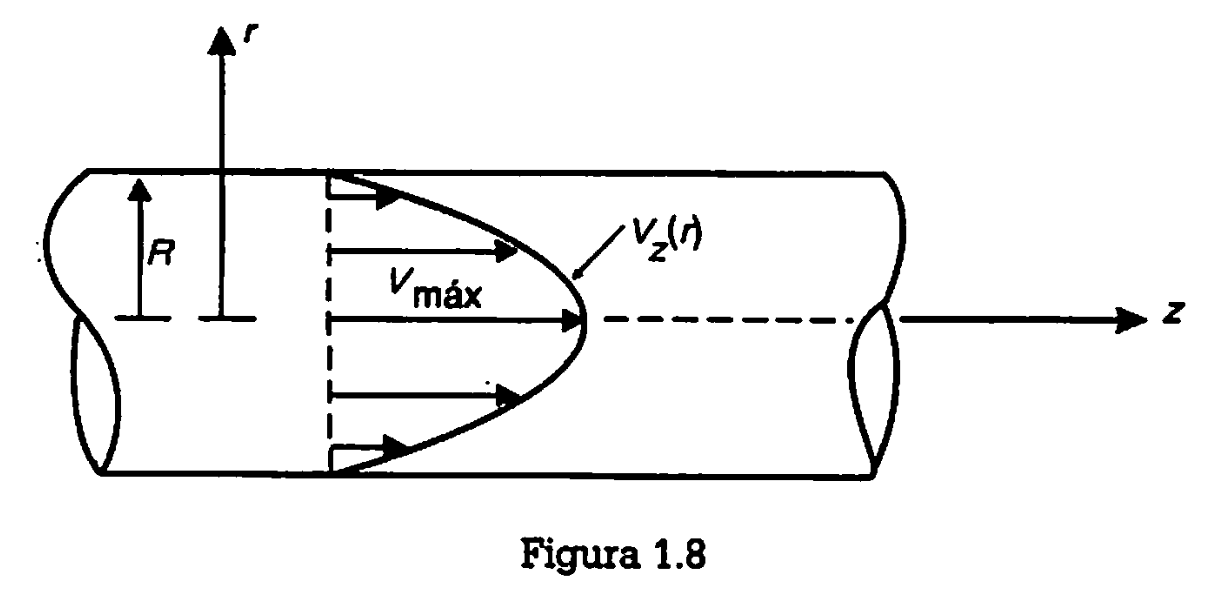
\includegraphics[height=\textheight]{images/Captura de tela de 2025-03-25 17-07-55.png}}
\end{frame}

\begin{frame}
    \begin{itemize}
        \item[1.6] A figura 1.9 mostra um esquema de um escoamento laminar, totalmente desenvolvido e em
            regime permanente, de um fluido newtoniano, entre duas placas paralelas e estacionárias, de 
            grandes dimensões e separadas de uma distância \(h\) pequena. A distribuição de velocidade
            de escoamento é dada por
            \[
                V_x (y) = V_\text{máx} \left[ 1-\left(\frac{2y}{h}\right)^2\right]
            \]

            Determine a força cisalhante, por unidade de área, exercida pelo escoamento sobre a placa superior.
    \end{itemize}
    \centering
    \vboxcorr{130pt}{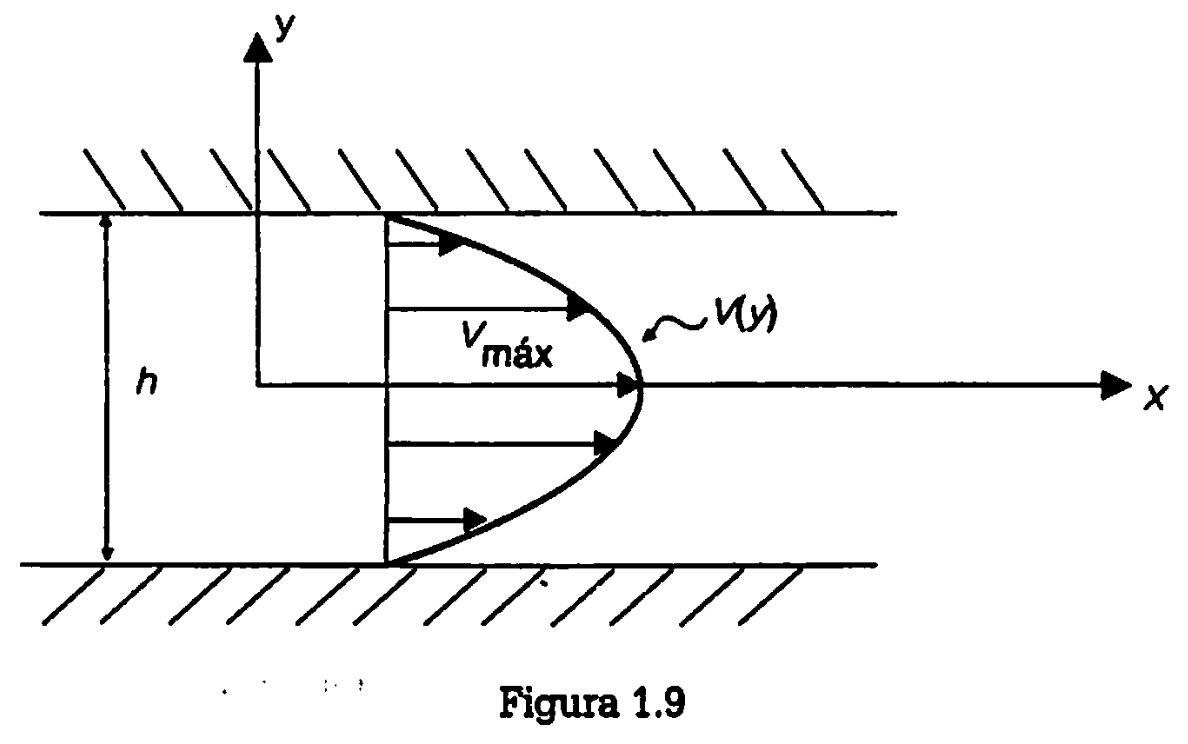
\includegraphics[height=\textheight]{images/Captura de tela de 2025-03-25 17-20-53.png}}
\end{frame}

\begin{frame}{Atividade 1}
    \begin{itemize}
        \item Vale 10\% da \(N_1\)
        \item Individual
        \item Leia as seções 1.8 e 1.9 do livro texto
        \item Resolva os problemas 1.7, 1.8, 1.9 e 1.10
        \item Data de entrega: 11/04/2025
        \item Google Sala de Aula: 
            https://classroom.google.com/c/NzYyNDc5OTQ1OTUx?cjc=\textcolor{blue}{mvcaim6v}
    \end{itemize}
\end{frame}

\begin{frame}[c]{Algumas unidades \textit{diferentes}}
    \begin{columns}
        \begin{column}{0.45\textwidth}
            \centering
            Viscosidade dinâmica
            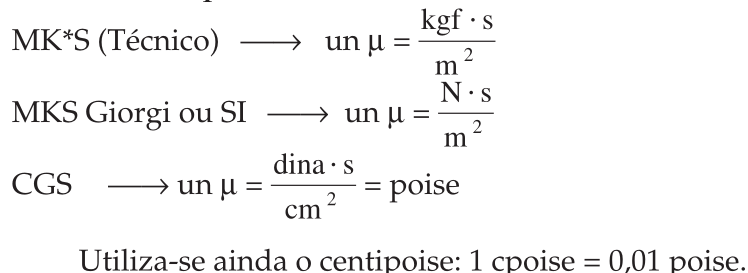
\includegraphics[width=\textwidth]{images/Captura de tela de 2025-03-26 16-53-52.png}
        \end{column}

        \begin{column}{0.45\textwidth}
            \centering
            Viscosidade cinemática
            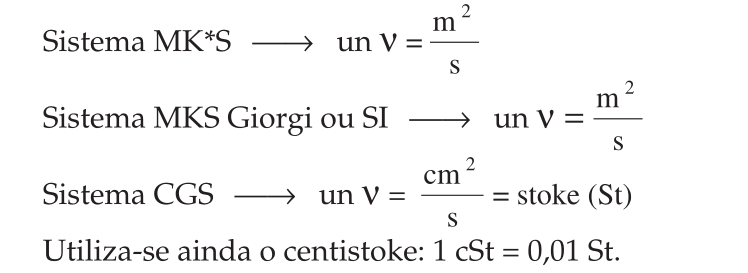
\includegraphics[width=\textwidth]{images/Captura de tela de 2025-03-26 16-54-30.png}
        \end{column}
    \end{columns}
\end{frame}
\begin{frame}{Exercícios do Livro Mecânica dos Fluidos de Franco Brunneti}
    \centering
    \includegraphics<+>[width=\textwidth]{images/Captura de tela de 2025-03-26 16-46-29.png}

    \includegraphics<+>[width=\textwidth]{images/Captura de tela de 2025-03-26 16-48-04.png}

    \includegraphics<+>[width=\textwidth]{images/Captura de tela de 2025-03-26 16-48-17.png}

    \includegraphics<+>[width=\textwidth]{images/Captura de tela de 2025-03-26 17-03-32.png}

    \only<.>{\vboxcorr{15pt}{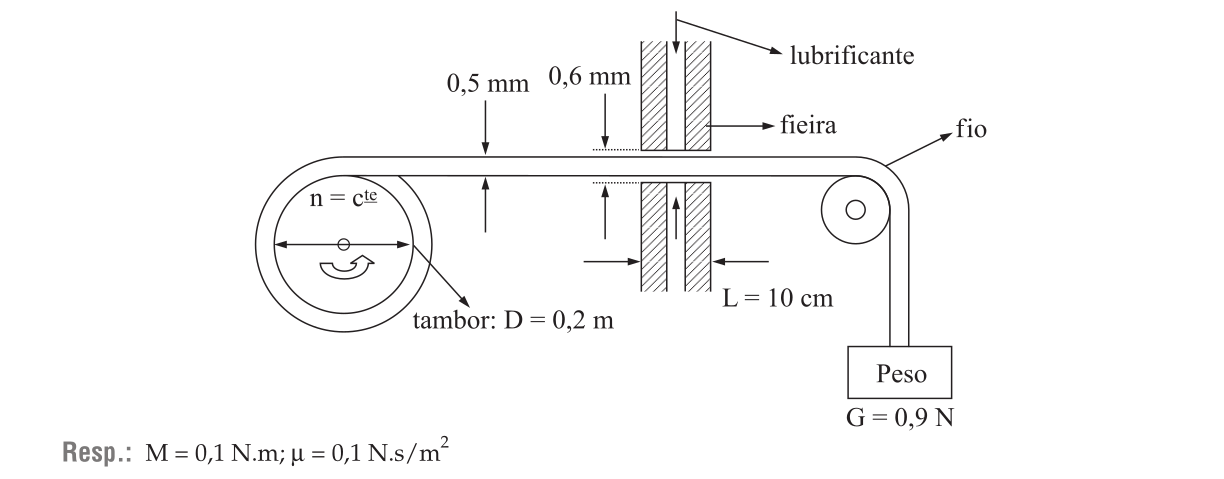
\includegraphics[width=\textwidth]{images/Captura de tela de 2025-03-26 17-03-50.png}}}

    \includegraphics<+>[width=\textwidth]{images/Captura de tela de 2025-03-26 16-37-14.png}

    \only<+>{\vboxcorr{23pt}{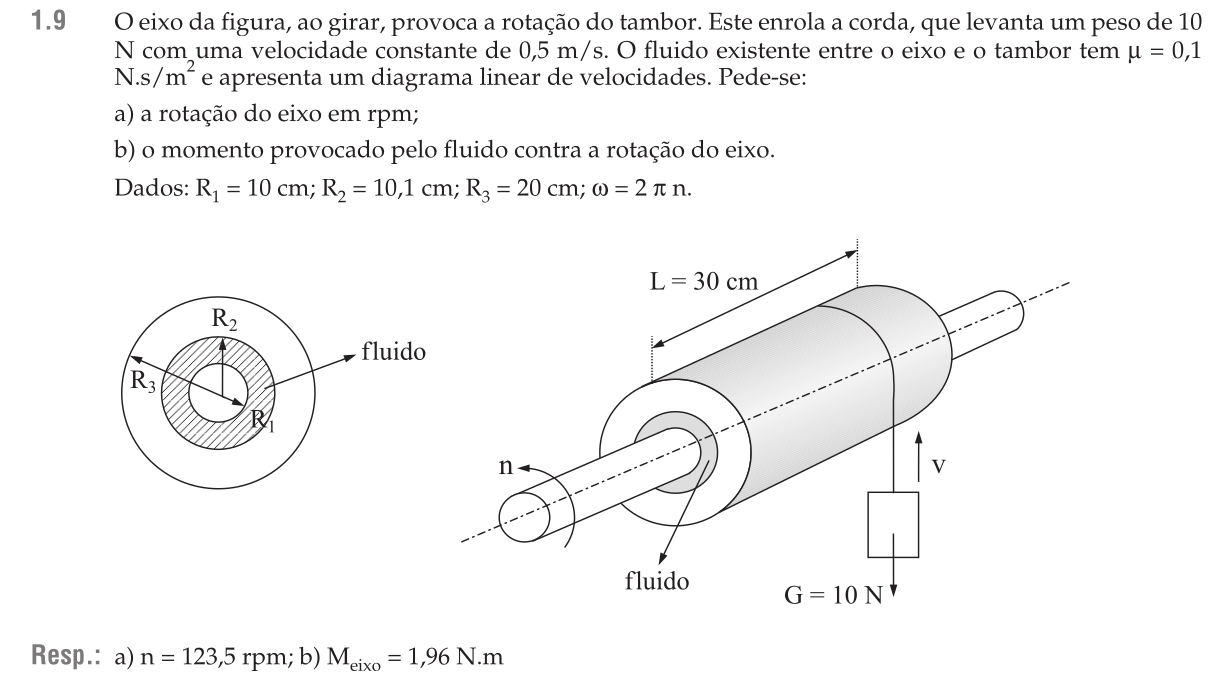
\includegraphics[width=\textwidth]{images/Captura de tela de 2025-03-26 17-07-59.png}}}

    \only<+>{\vboxcorr{2pt}{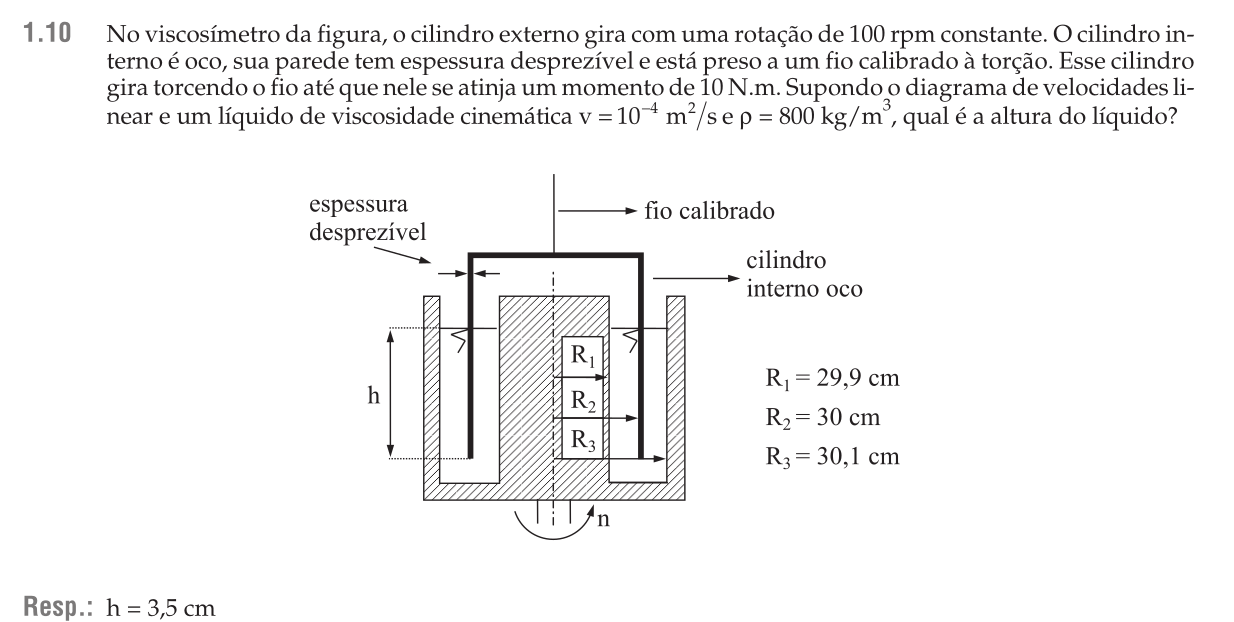
\includegraphics[width=\textwidth]{images/Captura de tela de 2025-03-26 17-22-38.png}}}

\end{frame}

 \begin{frame}{Revisão de Física Geral II}
     \centering 
     \includegraphics<+>[height=\textheight-28pt]{images/Captura de tela de 2025-04-01 15-36-19.png}

     \includegraphics<+>[height=\textheight-28pt]{images/Captura de tela de 2025-04-01 16-47-54.png}

     \includegraphics<+>[height=\textheight-28pt]{images/Captura de tela de 2025-04-01 15-37-11.png}

     \includegraphics<+>[height=\textheight-28pt]{images/Captura de tela de 2025-04-01 15-37-52.png}

 \end{frame}

 \begin{frame}{Revisão de Física Geral II}
     \begin{columns}[T]
         \begin{column}{0.45\textwidth}
             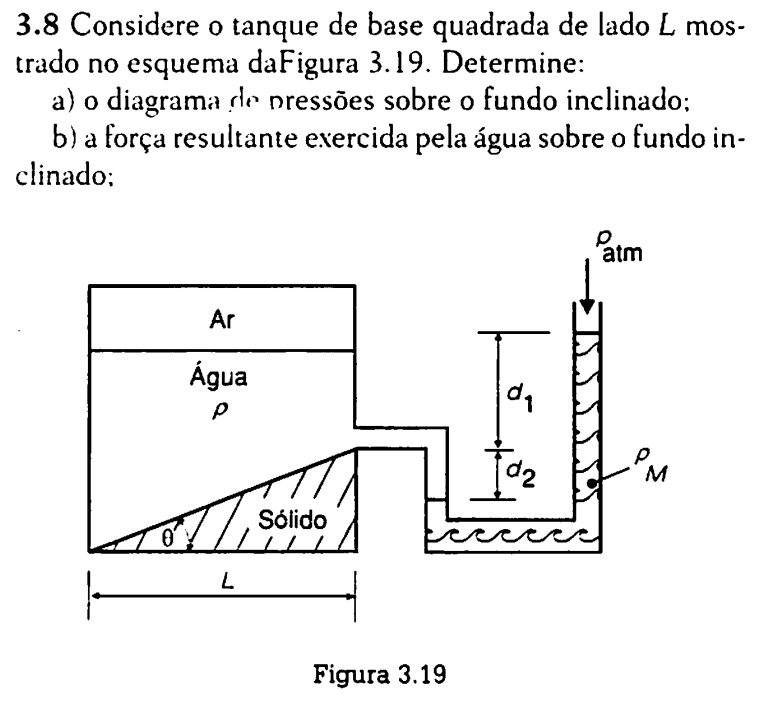
\includegraphics[width=\textwidth]{images/Captura de tela de 2025-04-01 15-55-30.png}
         \end{column}
%%%%%%%%%%%%%%%%%%%%%%%%%%%%%%%%%%%%%%%%%%%%%%%%%%
         \begin{column}{0.45\textwidth}

             \begin{tikzpicture}
                 \node [inner sep=0] (A) {
                     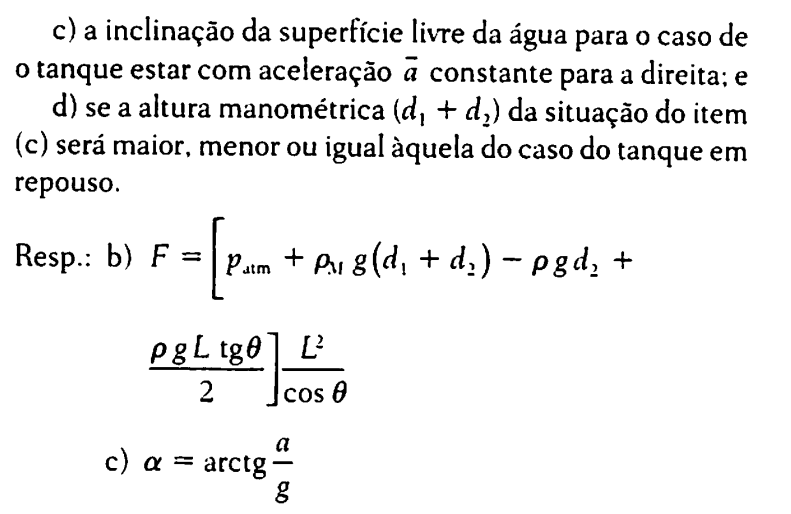
\includegraphics[width=\textwidth]{images/Captura de tela de 2025-04-01 15-55-44.png}
                 };


                 \coordinate (X0) at ($(A.south west)!0.00!(A.south east)$);
                 \coordinate (X1) at ($(A.south west)!0.99!(A.south east)$);
                 \coordinate (Y0) at ($(A.north west)!0.02!(A.south west)$);
                 \coordinate (Y1) at ($(A.north west)!0.40!(A.south west)$);
                 \filldraw [red, opacity=0.1] (X0|-Y0) rectangle (X1|-Y1);
             \end{tikzpicture}
         \end{column}
     \end{columns}
 \end{frame}


 \begin{frame}{Revisão de Física Geral II}
     \begin{columns}[T]
         \begin{column}{0.5\textwidth}
             \vboxcorr{44pt}{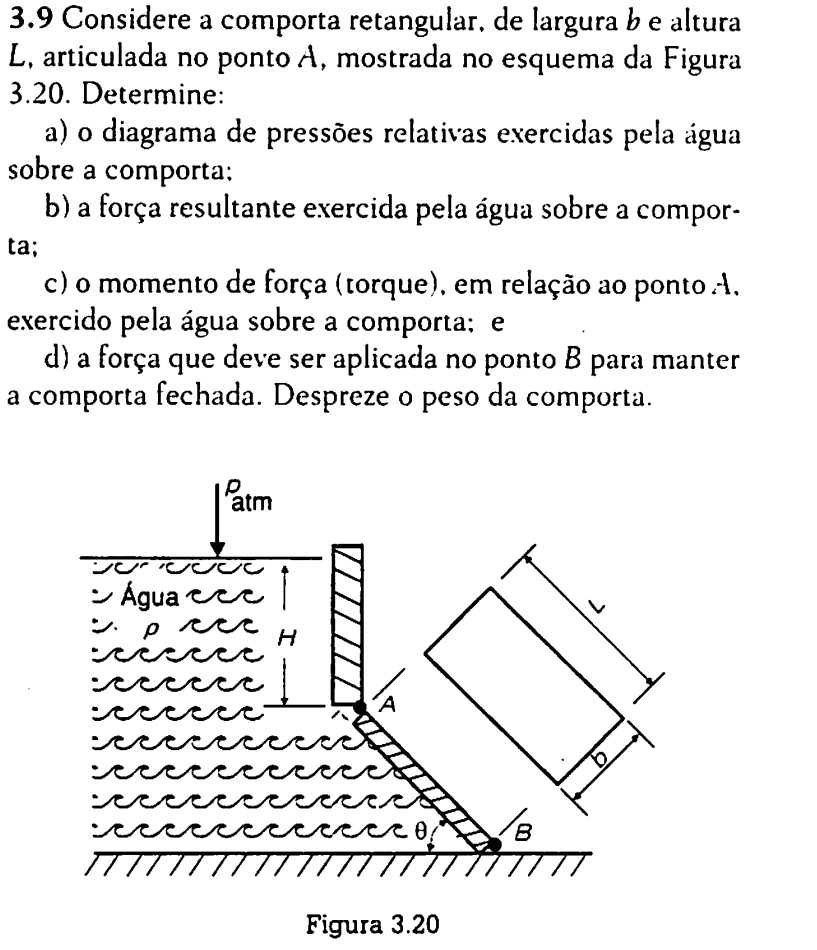
\includegraphics[width=\textwidth]{images/Captura de tela de 2025-04-01 17-06-56.png}}
         \end{column}

         \begin{column}{0.4\textwidth}
             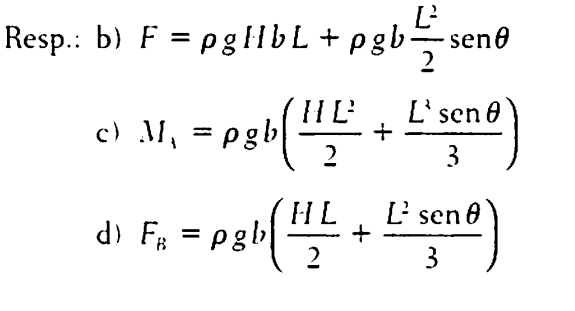
\includegraphics[width=\textwidth]{images/Captura de tela de 2025-04-02 16-47-44.png}
         \end{column}
     \end{columns}
 \end{frame}

 \begin{frame}<1>[label=bob1]{Revisão de Física Geral II}
     \centering
     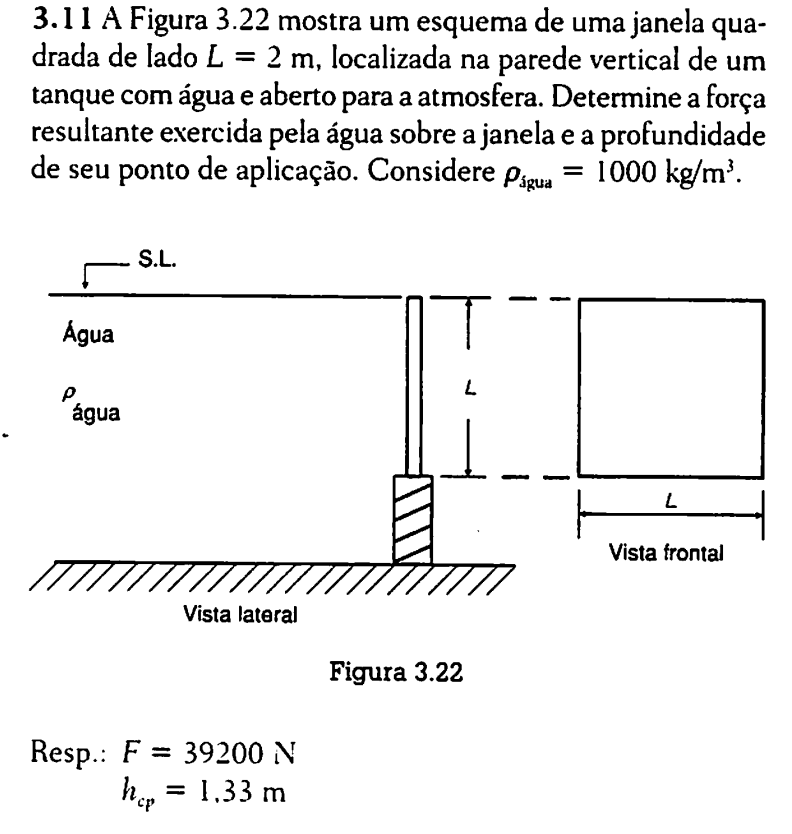
\includegraphics[height=\textheight-28pt]{images/Captura de tela de 2025-04-02 16-54-56.png}
 \end{frame}

 \begin{frame}<1>[label=bob2]{Revisão de Física Geral II}
     \begin{columns}[T]
         \begin{column}{0.5\textwidth}
             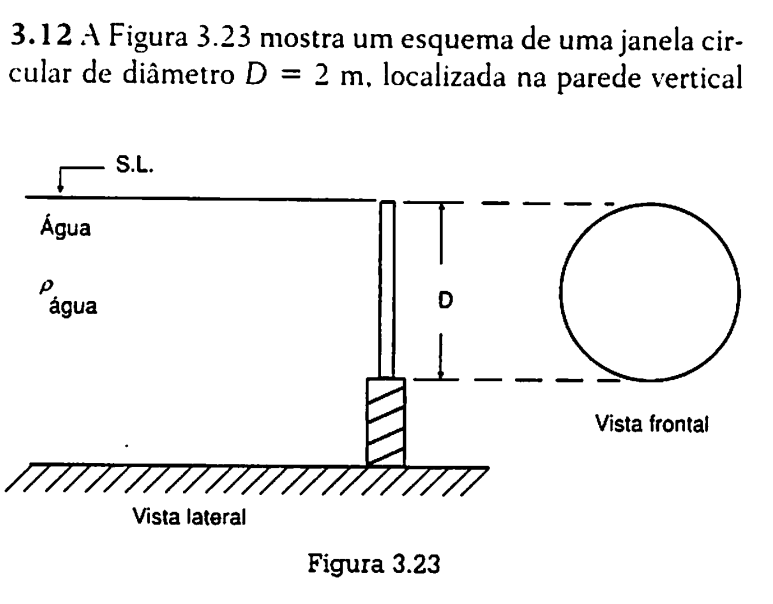
\includegraphics[width=\textwidth]{images/Captura de tela de 2025-04-02 16-55-06.png}
         \end{column}

         \begin{column}{0.4\textwidth}
             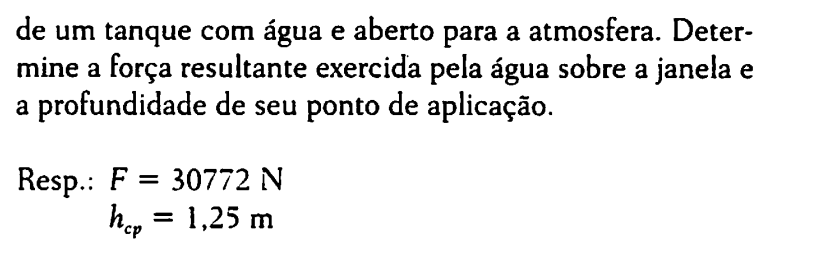
\includegraphics[width=\textwidth]{images/Captura de tela de 2025-04-02 16-55-20.png}
         \end{column}
     \end{columns}
 \end{frame}

 \begin{frame}{Resolução da 3.12}
     \begin{columns}[T]
         \begin{column}{0.4\textwidth}
             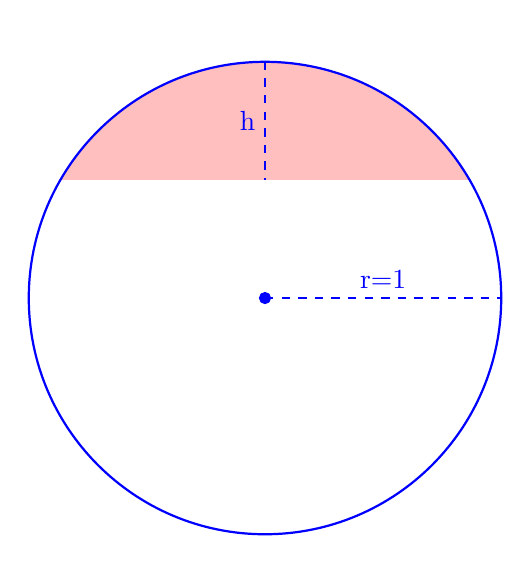
\begin{tikzpicture}
                 \filldraw [red!25] (0,0) ++(150:3cm) arc (150:30:3cm);
                 \filldraw [blue] (0,0) circle (2pt);
                 \draw [blue, dashed] (0,0) -- node [above, midway] {r=1} (3cm,0);
                 \draw [blue, dashed] (0,3cm) -- node[left,midway] {h} (0,1.5cm) ;
                 \draw [blue, thick] (0,0) circle (3cm);
             \end{tikzpicture}
         \end{column}
        %%%%%%%%%%%%%%%%%%%%%%%%%%%%%%%%%%%%%%%%%%%%%%%%%% 
         \begin{column}{0.55\textwidth}
             \textit{Facilmente}\footnote{Na atividade essas contas devem ser explicadas: regra da cadeia
             e do produto para a derivada e substituição trigonométrica para as integrais} podemos 
             encontrar
             \begin{align*}
                 & A=\arccos{(1-h)}-(1-h)\sqrt{1-(1-h)^2} \\
                 & dA = 2\sqrt{2h - h^2}dh \\
                 & \int_0^2 2 h\sqrt{2h-h^2}\; dh = \pi \\
                 & \int_0^2 2 h^2\sqrt{2h-h^2}\; dh =\frac{5\pi}{4} \\
                 & F = 9.8 \times 1000 \times \pi = \SI{30787.6}{N} \\
                 & F h_{cp} = \tau \implies h_{cp} = \frac{5}{4} = \SI{1.25}{m}
             \end{align*}
         \end{column}
     \end{columns}
 \end{frame}

\begin{frame}{Forma \textit{mais simples} para calcular \(F\) e \(h_{cp}\)}
    \begin{itemize}
        \item Na seção 2.10 do livro do Brunetti é demonstrado que a força
            \(F\) sobre uma superfície plana submersa é dada por
            \[
                F = \bar{p}{A}
            \]
            onde \(\bar{p}\) é a pressão no centro de gravidade CG \footnote{Centro de massa se
            a gravidade é constante} e \(A\) é a área da superfície
        \item Já na seção 2.11 do mesmo livro é demonstrado que a posição
            vertical do centro de pressão (\(h_{cp}\)) é dada por
            \[
                h_{cp} = \bar{h}+\frac{\bar{I}}{\bar{h}A}
            \]
            onde \(\bar{h}\) é a posição do CG, \(\bar{I}\) é o momento de inércia
            calculado em relação a um eixo que passa pelo CG da superfície
    \end{itemize}
\end{frame}

\begin{frame}
    \centering
    \vboxcorr{22pt}{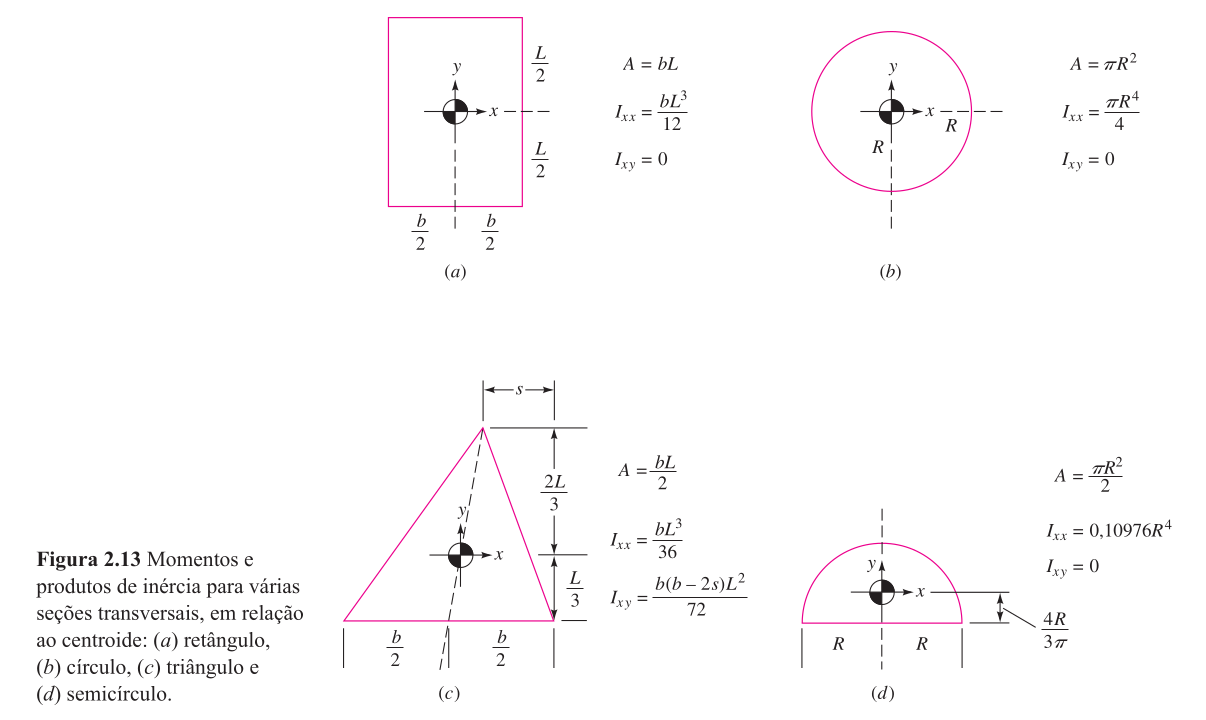
\includegraphics[width=\textwidth]{images/Captura de tela de 2025-04-09 17-26-36.png}}
\end{frame}

\againframe<2->{bob1}
\againframe<2->{bob2}

\begin{frame}{Revisão de Física Geral II}
     \centering
     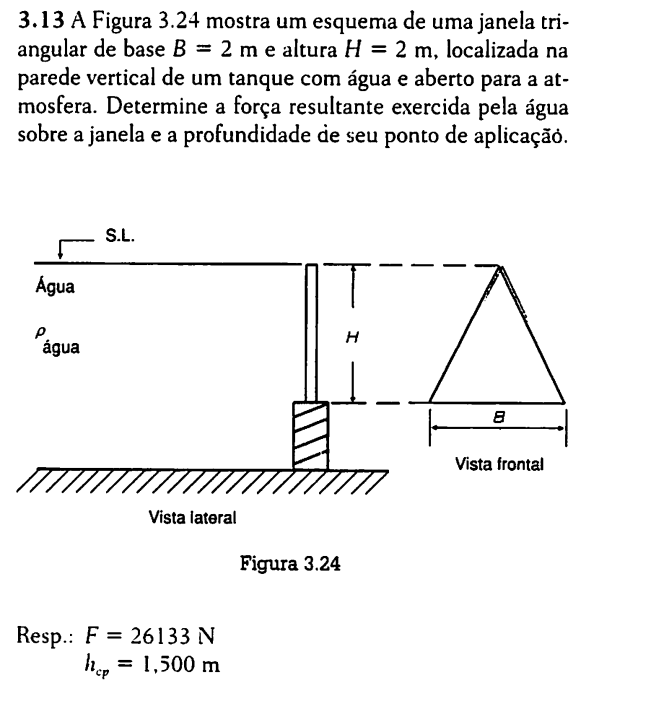
\includegraphics[height=\textheight-28pt]{images/Captura de tela de 2025-04-08 17-54-32.png}
\end{frame}

\begin{frame}{Revisão de Física geral II}
     \centering
     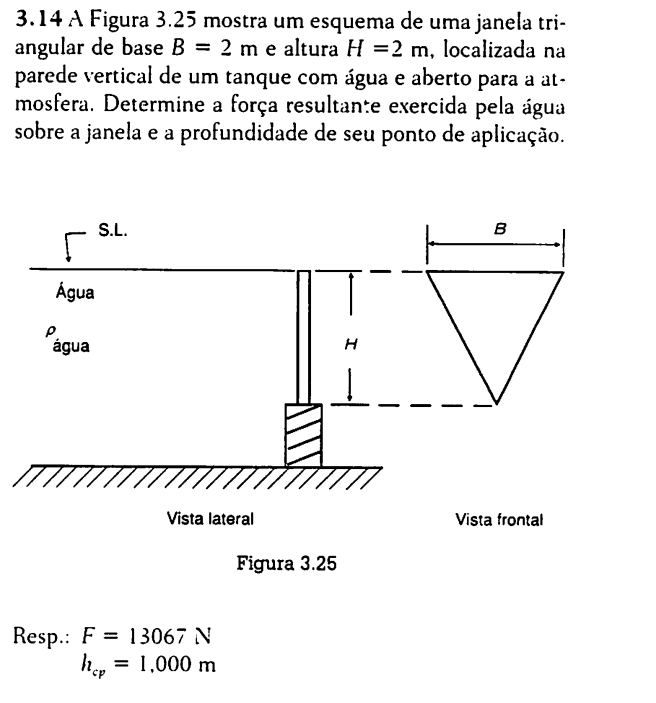
\includegraphics[height=\textheight-28pt]{images/Captura de tela de 2025-04-08 17-54-50.png}
\end{frame}

\begin{frame}{Revisão de Física geral II}
    \begin{columns}[T]
        \begin{column}{0.45\textwidth}
            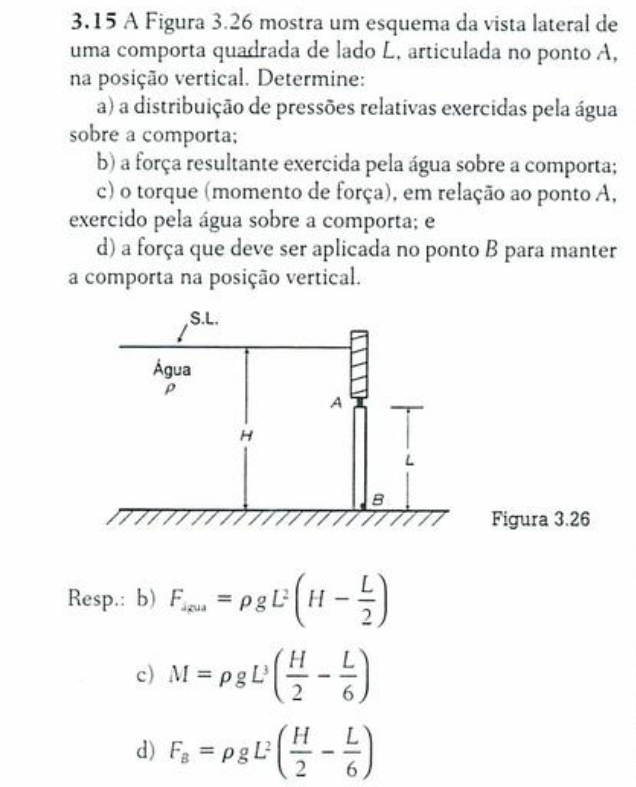
\includegraphics[height=\textheight-35pt]{images/Captura de tela de 2025-04-08 17-56-49.png}
        \end{column}
        %%%%%%%%%%%%%%%%%%%%%%%%%%%%%%%%%%%%%%%%%%%%%%%%%%
        \begin{column}{0.45\textwidth}
            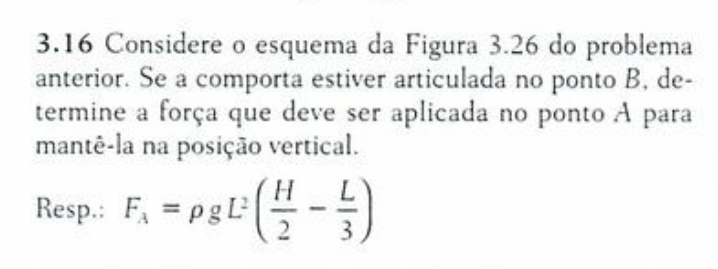
\includegraphics[width=\textwidth]{images/Captura de tela de 2025-04-09 16-46-12.png}
        \end{column}
    \end{columns}
\end{frame}

% \begin{frame}{Revisão de Física geral II (livro do White)}
%     \centering
%     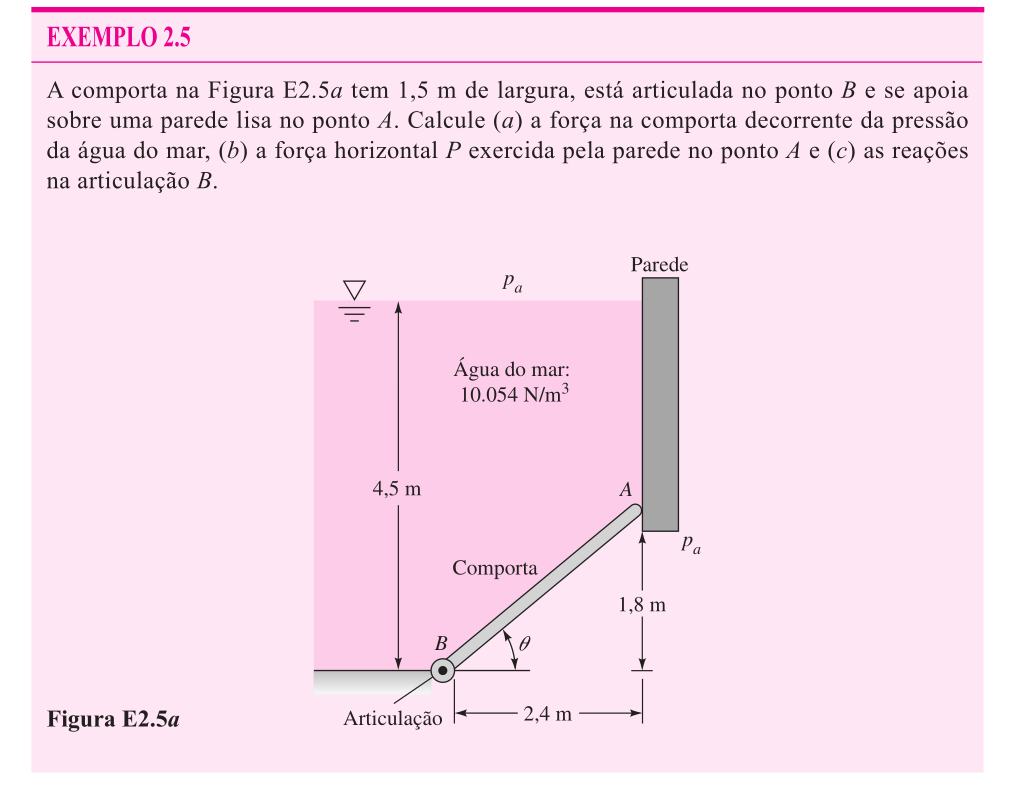
\includegraphics[height=\textheight-28pt]{images/Captura de tela de 2025-04-09 17-32-25.png}
% \end{frame}


\begin{frame}{Classificação de escoamentos}
    \begin{itemize}
        \item No escoamento laminar, o movimento do fluido se passa como se o
            fluido tosse constituído de lâminas paralelas que deslizam umas em
            relação às outras, sem ocorrer mistura macroscópica.
        \item No escoamento turbulento, as partículas fluidas se movem em
            trajetórias irregulares e ocorre mistura macroscópica
        \item O tipo de escoamento pode ser ''determinado'' através do \textit{número de Reynolds}
            \[
                \text{Re} = \frac{\rho V D}{\mu}
            \]
            onde \(\rho\) é a massa específica do fluido, \(V\) é a velocidade média
            de escoamento no duto, \(D\) é o diâmetro interno do duto e \(\mu\)
            é a viscosidade dinâmica do fluido

        \item A velocidade média é dada por
            \[
                V=\frac{Q}{A}
            \]
            onde \(Q\) é a vazão volumétrica e \(A\) é a área da seção transversal do tubo
    \end{itemize}
\end{frame}

\begin{frame}
    \begin{itemize}
        \item<+-> Por exemplo, para o escoamento por um tubo de \SI{5}{cm} de
            diâmetro a que vazão volumétrica temos \(\text{Re} = 2300\) para (a) ar e
            (b) água?
        \item<+-> Sabendo que para o ar \(\rho=\SI{1.205}{kg/m^3}\) e
            \(\mu = \SI{1.80e-5}{kg/m\cdot s}\), temos \(Q \approx \SI{350}{m^3/s}\)
        \item<+-> Sabendo que para água \(\rho=\SI{998}{kg/m^3}\) e
            \(\mu = \SI{1e-3}{kg/m\cdot s}\), temos \(Q \approx \SI{23.5}{m^3/s}\)

        \item<+-> Para \(\text{Re} < 2100\), o escoamento, em geral, é laminar 

        \item<.-> Para \(\text{Re} > 2500\), ocorre escoamento turbulento

        \item<.-> Para \(2100 < \text{Re} < 2500\) o escoamento pode ser laminar ou
            turbulento em função das condições ambientes, principalmente da
            presença de vibrações no sistema
    \end{itemize}
\end{frame}

\begin{frame}{Escoamento de entrada e estabelecido em um duto}
    \centering
    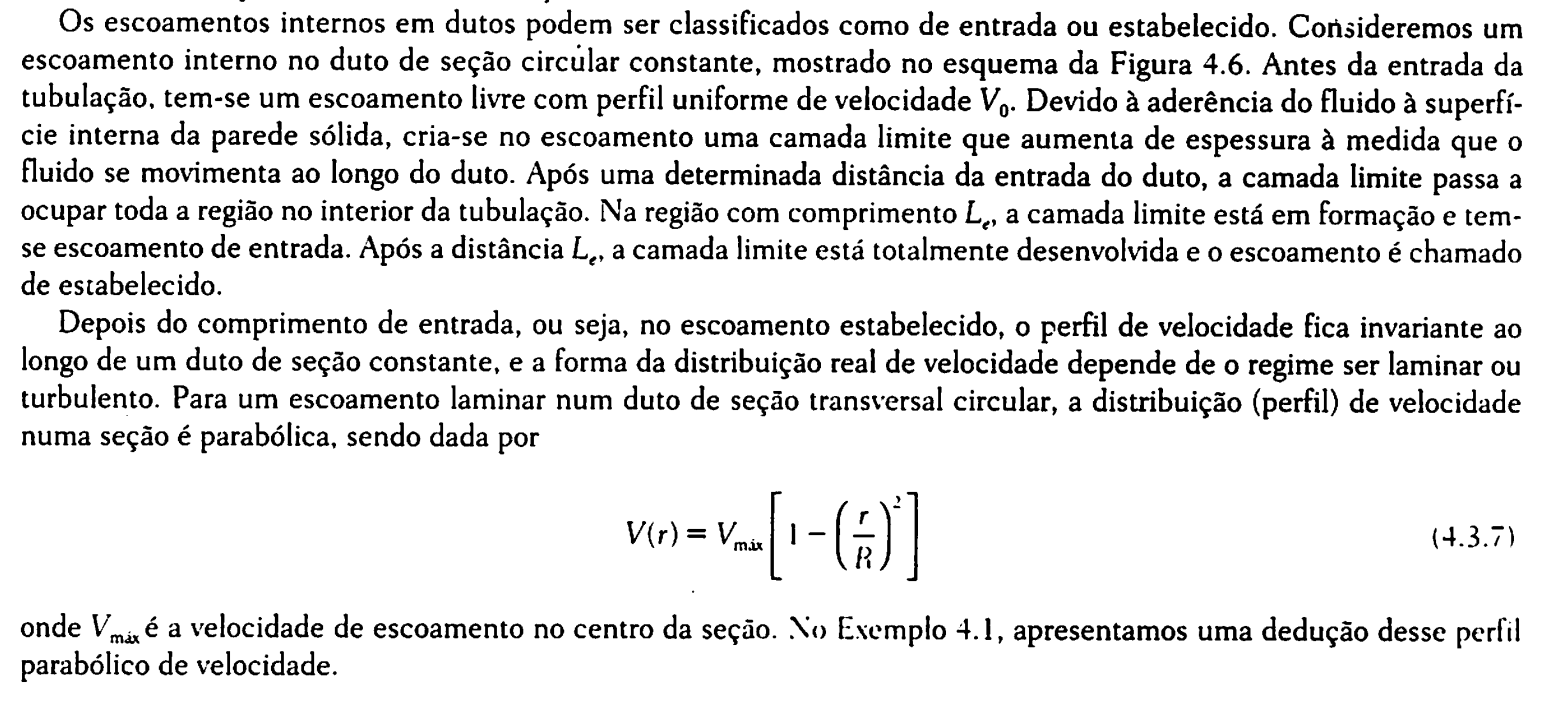
\includegraphics[width=\textwidth]{images/Captura de tela de 2025-04-15 16-23-56.png}
\end{frame}

\begin{frame}
    \centering
    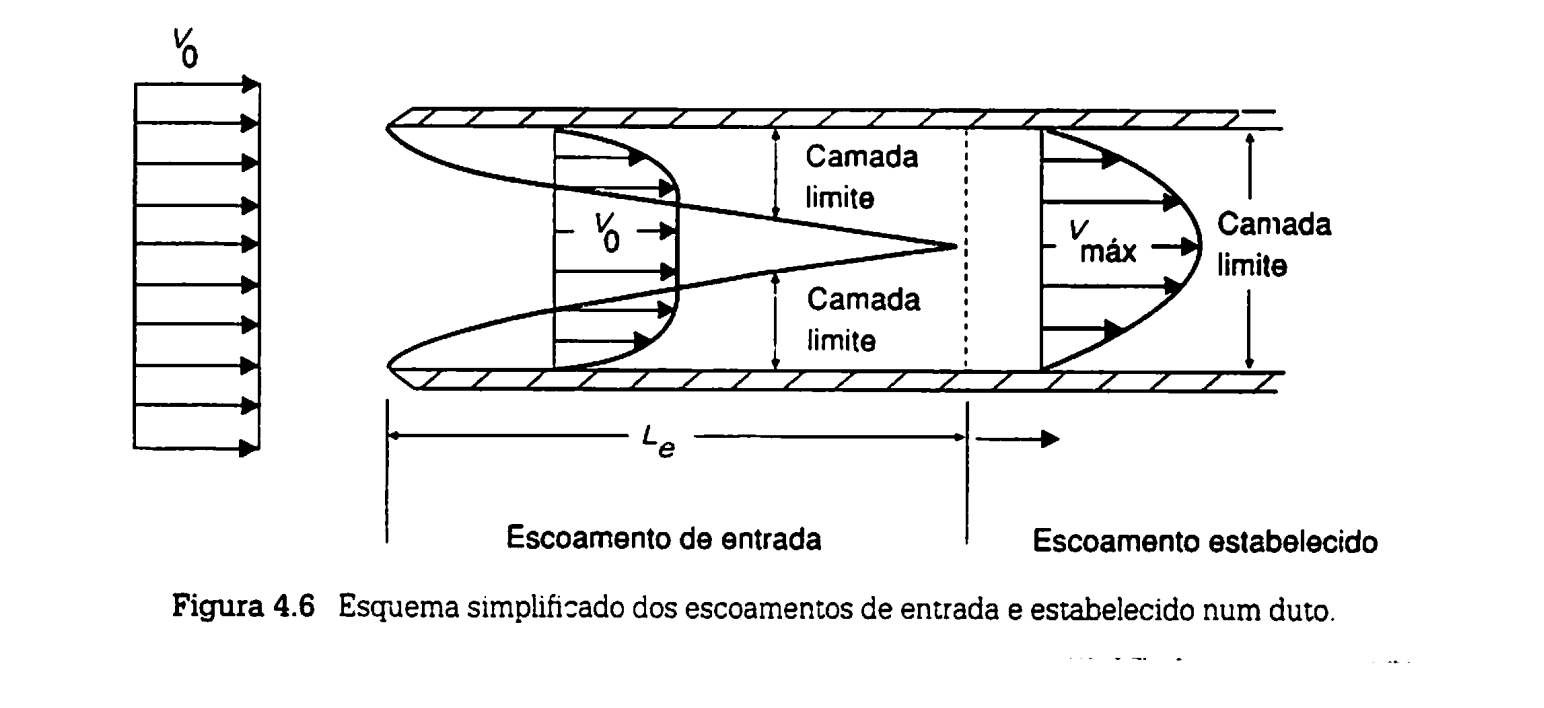
\includegraphics[width=\textwidth]{images/Captura de tela de 2025-04-15 16-26-48.png}
\end{frame}

\begin{frame}{Exemplo 4.1: dedução da equação 4.3.7}
    \begin{itemize}
        \item Seja um elemento de volume fluido cilíndrico

            \begin{center}
                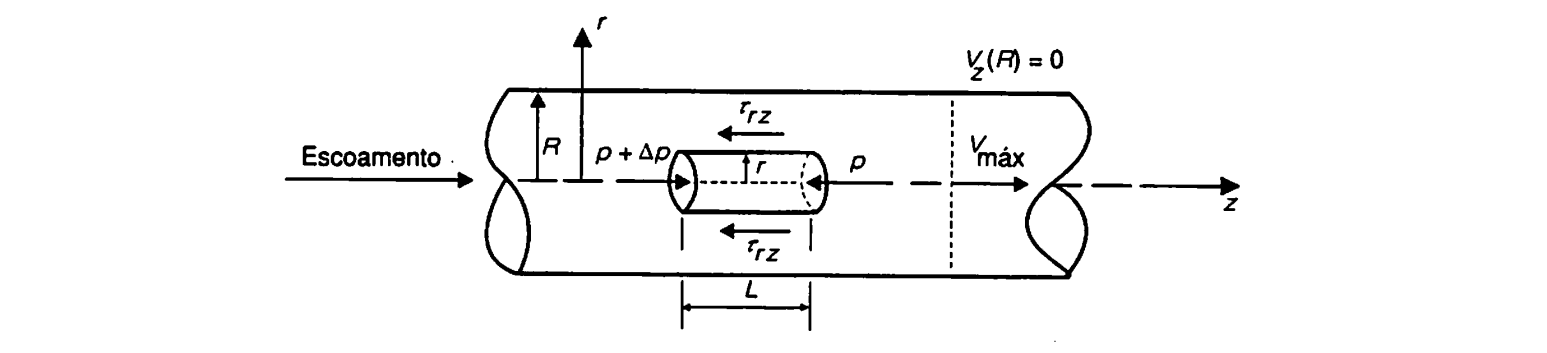
\includegraphics[width=\textwidth-25pt]{images/Captura de tela de 2025-04-15 16-33-57.png}
            \end{center}

        \item Sobre ele atuam a força resultante de pressão que causa o escoamento e
            força de atrito viscoso devido às tensões cisalhantes
            \[
                \sum F_z = \Delta p \pi r^2 - 2\pi r L \tau_{rz} = 0 \implies 
                \tau_{rz} =\frac{\Delta p}{2L} r = \alert<2->{-}\mu \frac{d V}{d r}
            \]
            onde \(V(r=0) \equiv V_\text{máx}\) e \(V(r=R) \equiv 0\)
        \item Resolvendo a EDO encontramos \textit{facilmente} a equação 4.3.7

    \end{itemize}
\end{frame}

\begin{frame}{Fim do assunto para a 1\esima{} prova}
    Lista de exercícios:
    \begin{itemize}
        \item Problemas 1.3, 1.5 e 1.6 do livro texto (Celso Livi)
        \item Problemas 1.4, 1.5, 1.6, 1.7, 1.8, 1.9 e 1.10 do livro auxiliar (Franco Brunneti)
        \item Problemas 3.1, 3.3, 3.4, 3.5, 3.8b, 3.9, 3.11, 3.12, 3.13, 3.14 e 3.15 do livro texto
    \end{itemize}

    A prova terá entre 3 e 4 problemas da lista com \textit{valores numéricos modificados}
\end{frame}

\newcommand{\volume}{{\ooalign{\hfil$V$\hfil\cr\kern0.08em--\hfil\cr}}}
\begin{frame}{Vazão e fluxo de massa}
    \begin{itemize}
        \item O volume de fluido que escoa através de uma seção de área \(A\),
            no intervalo \(dt\), é dada por
            \[
                d\volume = \left[\iint\limits_A(\vec{V}\cdot\hat{n})\;dA\right]\;dt
            \]
        \item A vazão \(Q\) é o volume de fluido que escoa através da seção por unidade de tempo, ou seja
            \[
                Q=\iint\limits_A(\vec{V}\cdot\hat{n})\;dA
            \]
        \item O fluxo de massa \(\dot{m}\) é a massa de fluido que escoa
            através da seção por unidade de tempo, ou seja
            \[
                \dot{m}=\iint\limits_A\rho(\vec{V}\cdot\hat{n})\;dA
            \]
    \end{itemize}
\end{frame}

\begin{frame}{Exemplo 5.1}
    Determine a velocidade média, numa seção, de um escoamento laminar, totalmente
    desenvolvido e em regime permanente, no duto de seção circular com diâmetro
    constante mostrado no esquema da Figura 5.3

    \centering
    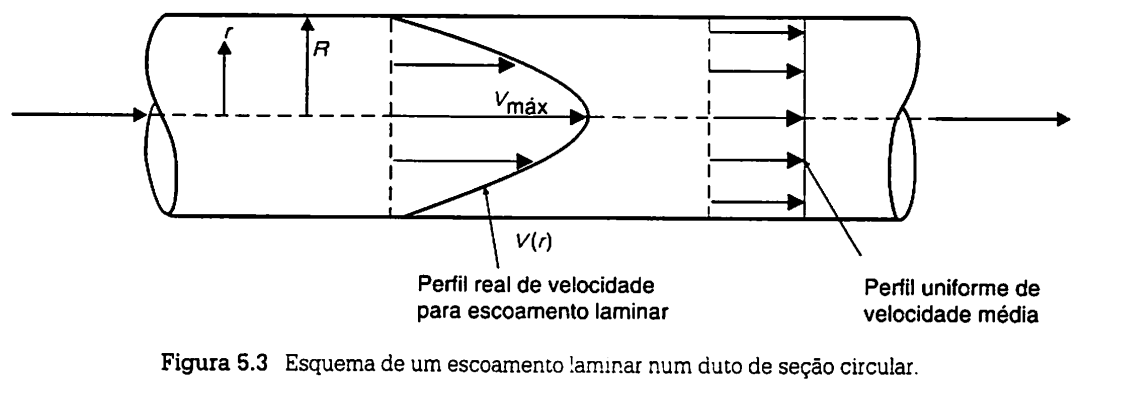
\includegraphics[width=\textwidth]{images/Captura de tela de 2025-04-23 17-09-17.png}
\end{frame}

\begin{frame}{Elemento de área de um círculo}
    \centering
    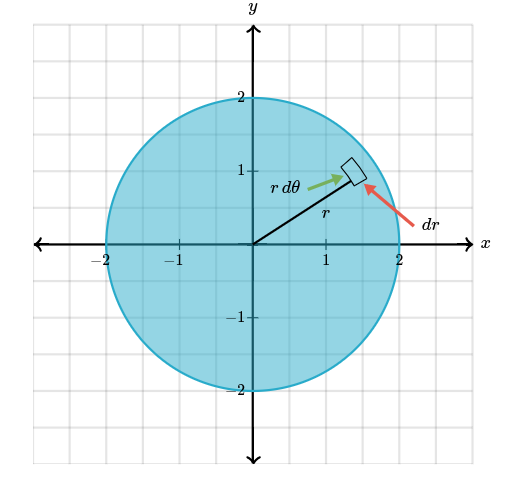
\includegraphics[height=\textheight-28pt]{images/Captura de tela de 2025-04-23 17-19-53.png}
\end{frame}

\begin{frame}{Exercício do Livro Mecânica dos Fluidos de Franco Brunneti}
    \centering
    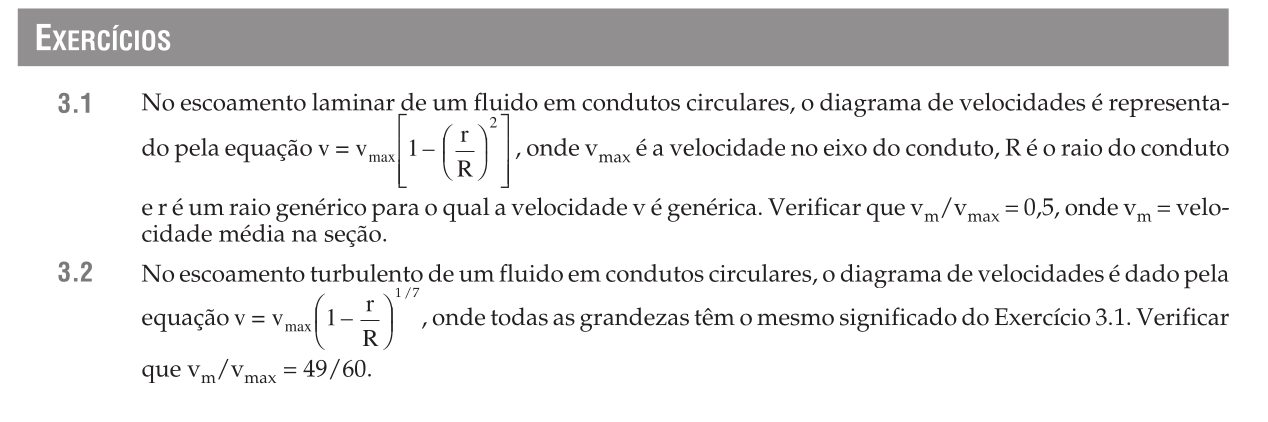
\includegraphics[width=\textwidth]{images/Captura de tela de 2025-04-23 17-58-33.png}
\end{frame}

\begin{frame}<1>[label=framb]{Exercícios}
    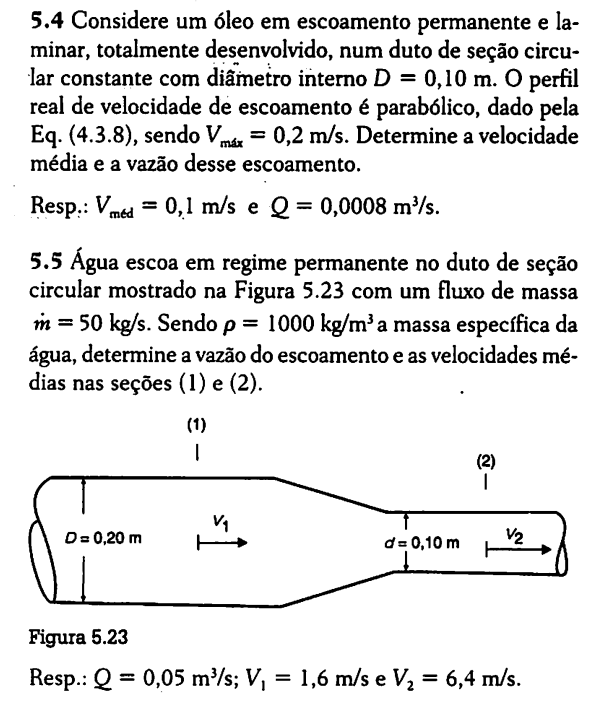
\includegraphics[height=\textheight-28pt]{images/Captura de tela de 2025-04-23 17-25-16.png}
\end{frame}


\begin{frame}{Equação de continuidade}
    \begin{itemize}
        \item Em regime permanente, as propriedades do fluido e as características 
            do escoamento ficam invariantes com o tempo (estacionárias)
        \item Dessa forma
            \[
                \int_\text{SC} \rho (\vec{V}\cdot\hat{n})\; dA = 0
            \]
            ou seja, \textit{a vazão total} atravessando a superfície de controle é zero
        \item Se \(\rho = \text{constante}\) e \(V = \text{constante}\), temos que
            \[
                Q_\text{total}= 0 \implies Q_\text{entrada}=Q_\text{saida}
            \]
    \end{itemize}
\end{frame}

\againframe<2->{framb}

\begin{frame}{Exercícios}
    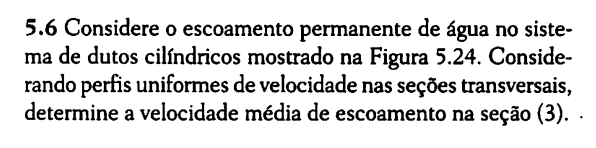
\includegraphics[height=0.3\textheight-14pt]{images/Captura de tela de 2025-04-23 17-29-10.png}

    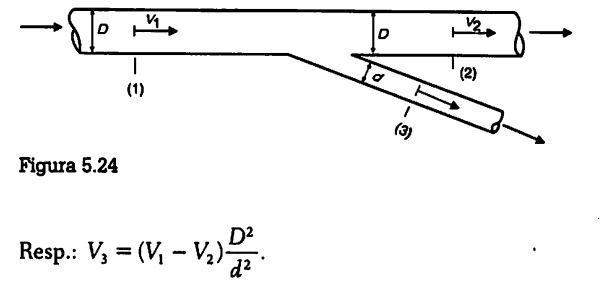
\includegraphics[height=0.5\textheight-14pt]{images/Captura de tela de 2025-04-23 17-29-19.png}
\end{frame}

\begin{frame}{Exercícios}
    \begin{columns}[T]
        \begin{column}{0.35\textwidth+19pt}
            \vboxcorr{7pt}{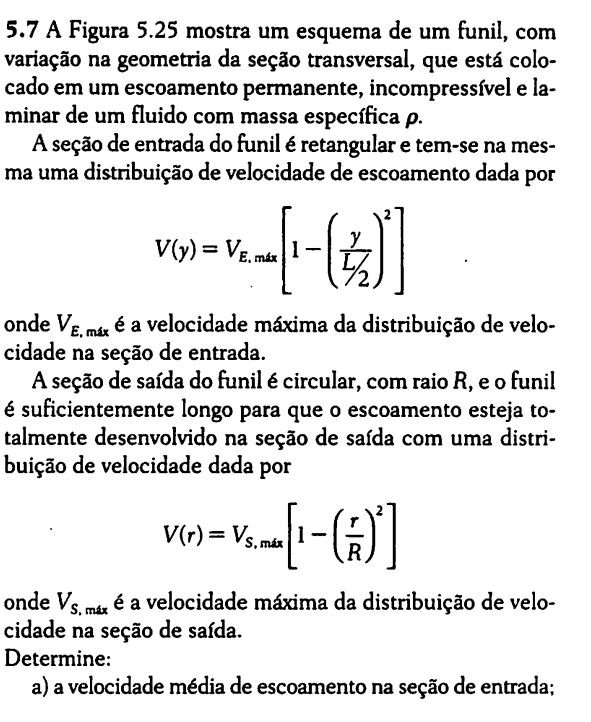
\includegraphics[height=\textheight-28pt]{images/Captura de tela de 2025-04-29 16-46-52.png}}
        \end{column}
        %%%%%%%%%%%%%%%%%%%%%%%%%%%%%%%%%%%%%%%%%%%%%%%%%%
        \begin{column}{0.35\textwidth+19pt}
            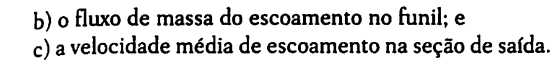
\includegraphics[width=\textwidth]{images/Captura de tela de 2025-04-29 16-47-12.png}
        \end{column}
    \end{columns}

\end{frame}

\begin{frame}{}
    \centering
    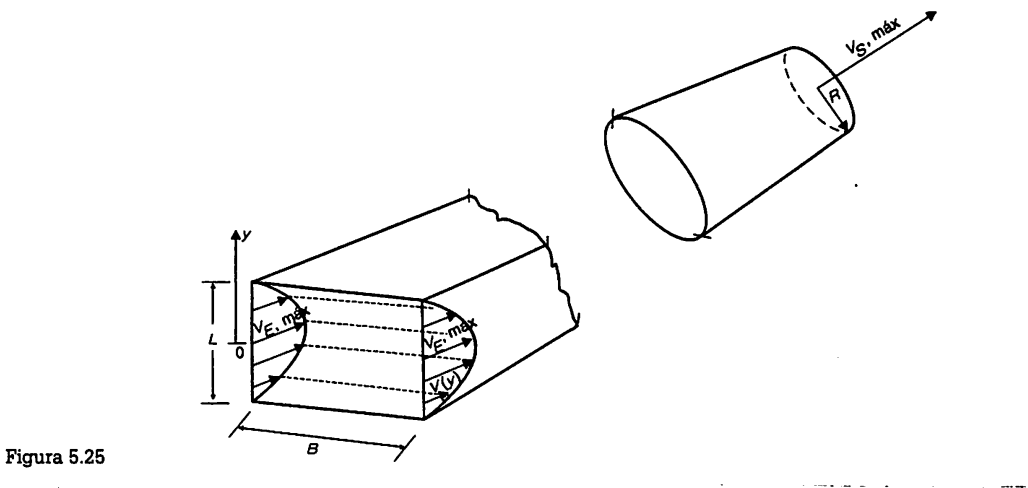
\includegraphics[width=\textwidth]{images/Captura de tela de 2025-04-29 16-47-32.png}
\end{frame}

\begin{frame}{Exercícios}
    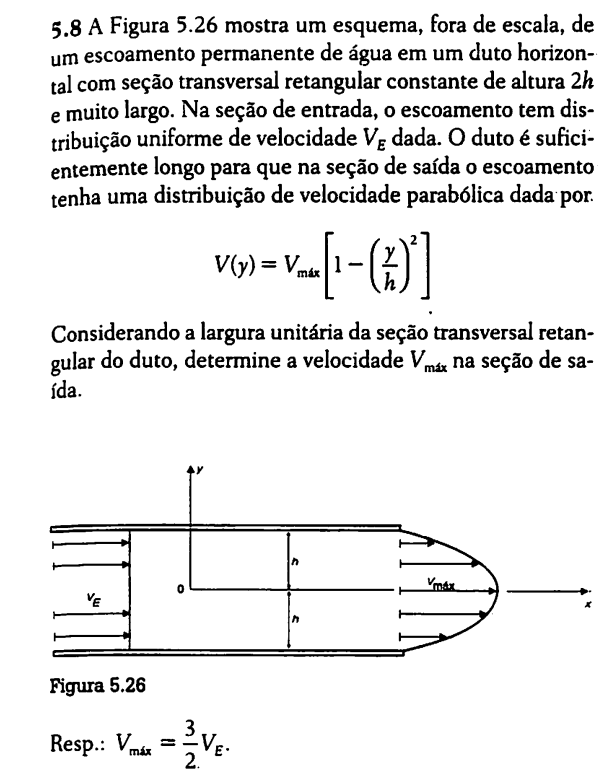
\includegraphics[height=\textheight-28pt]{images/Captura de tela de 2025-04-29 17-20-25.png}
\end{frame}

\begin{frame}{Exercício do Livro Mecânica dos Fluidos de Franco Brunneti}
    \centering
    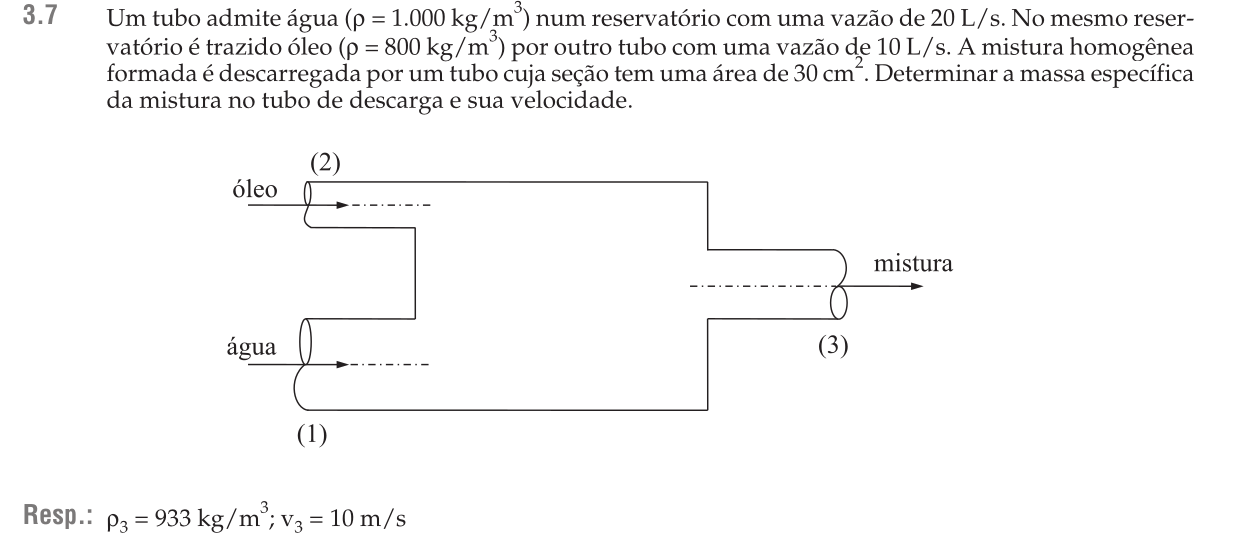
\includegraphics[width=\textwidth]{images/Captura de tela de 2025-04-29 17-26-04.png}
\end{frame}

\begin{frame}{Exercício do Livro Mecânica dos Fluidos de Franco Brunneti}
    \centering
    \vboxcorr{28pt}{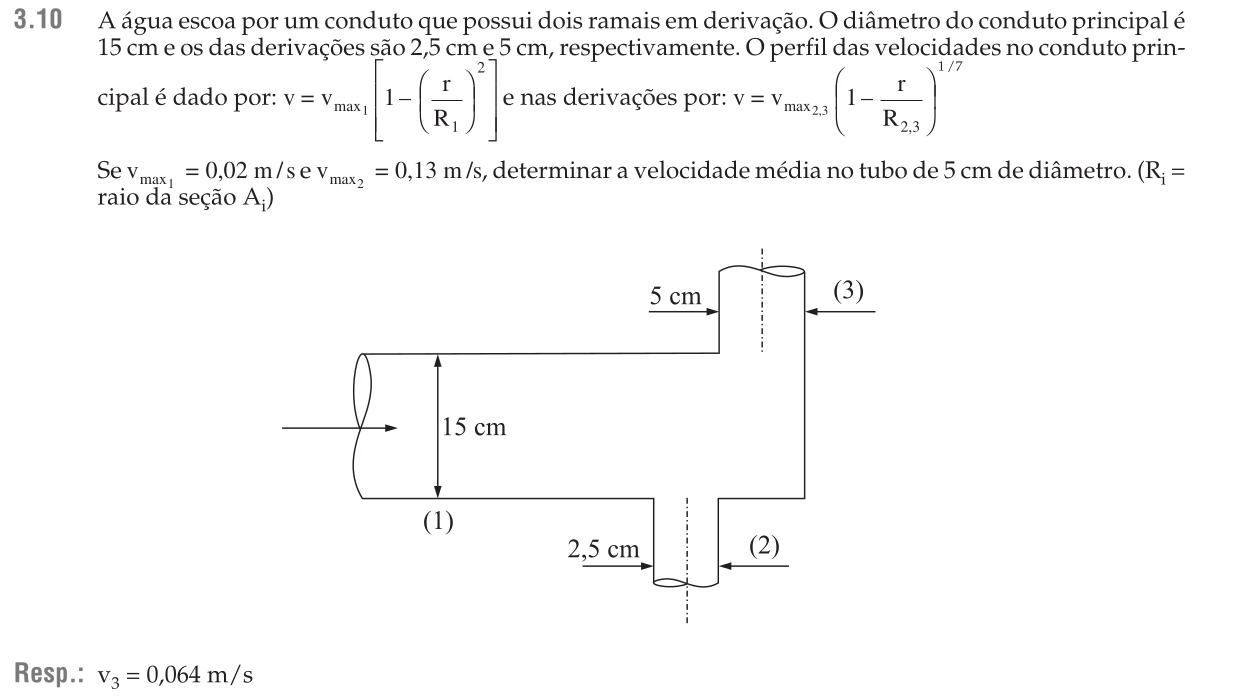
\includegraphics[width=\textwidth]{images/Captura de tela de 2025-04-29 17-35-44.png}}
\end{frame}

\begin{frame}{Equação de Bernoulli sem dissipação de energia mecânica}
    \[
        \rho g y_1 + \frac{1}{2} \rho V_1^2 + p_1 = 
        \rho g y_2 + \frac{1}{2} \rho V_2^2 + p_2
    \]
    \textit{Essa equação} expressa a conservação de energia mecânica
    ao longo de uma linha de corrente ou de um filete fluido (tubo de 
    corrente com seção transversal pequena) em um escoamento com as seguintes restrições:
    \begin{itemize}
        \item permanente
        \item fluido incompressível
        \item sem efeitos viscosos
        \item propriedades constantes nas seções transversais
        \item sem troca de calor
    \end{itemize}
\end{frame}

\begin{frame}{Equação de Bernoulli com perda de carga}
    \[
        y_1 + \frac{V_1^2}{2g}+\frac{p_1}{\rho g} = y_2 + \frac{V_2^2}{2g} + \frac{p_2}{\rho g}
        +h_p
    \]
    onde \(h_p\) é a perda de carga

    \textit{Essa equação} expressa a conservação de energia mecânica
    ao longo de uma linha de corrente ou de um filete fluido (tubo de 
    corrente com seção transversal pequena) em um escoamento com as seguintes restrições:
    \begin{itemize}
        \item permanente
        \item fluido incompressível
        \item propriedades constantes nas seções transversais
    \end{itemize}
\end{frame}

\begin{frame}{Perda de carga}
    \begin{itemize}
        \item A perda de carga \(h_p\) corresponde à parcela de energia
            mecânica do escoamento que é irreversivelmente convertida em
            energia térmica por causa do atrito viscoso 

        \item Considera-se a perda de carga total como a soma de dois tipos
            diferentes de perda de carga
            \begin{itemize}
                \item perda de carga distribuída \(h_{pd}\) devido ao atrito viscoso
                    ao longo da tubulação
                \item perda de carga localizada ou acidental \(h_{pl}\) devido aos
                    acessórios ou acidentes localizados em determinadas
                    posições nas tubulações, tais como válvulas, variações na
                    seção transversal, curvas, etc
            \end{itemize}
        \item A perda de carga distribuída pode ser calculada por meio da
            equação de Darcy-Weisbach, que pode ser escrita como
            \[
                h_{pd} = f\frac{L}{D}\frac{V_\text{média}^2}{2g}
            \]
            onde \(f\) é um coeficiente de proporcionalidade conhecido como \textit{fator de atrito},
            determinado experimentalmente, e
    \end{itemize}
\end{frame}

\begin{frame}{Fator de atrito}
    \begin{itemize}
        \item O fator de atrito é função de dois parâmetros unidimensionais
            \[
                f=f\left(\text{Re},\frac{e}{D}\right)
            \]
            onde Re é o número de Reynolds e \(e/D\) é a rugosidade relativa do duto
        \item A rugosidade da parede da tubulação \(e\) pode ser definida como a
            altura média das saliências da superfície interna do duto
        \item A rugosidade relativa \(e/D\) é o quociente entre a rugosidade e o diâmetro
            interno do duto

        \item Os fatores de atrito podem ser obtidos através do \textit{diagrama de Moody}
    \end{itemize}
\end{frame}

% \begin{frame}{Diagrama de Moody}
%     \centering
%     \def\svgwidth{\textwidth-100pt}
%     \input{Moody_EN.pdf_tex}
% \end{frame}

\begin{frame}{Diagrama de Moody}
    \centering
    \vboxcorr{82pt}{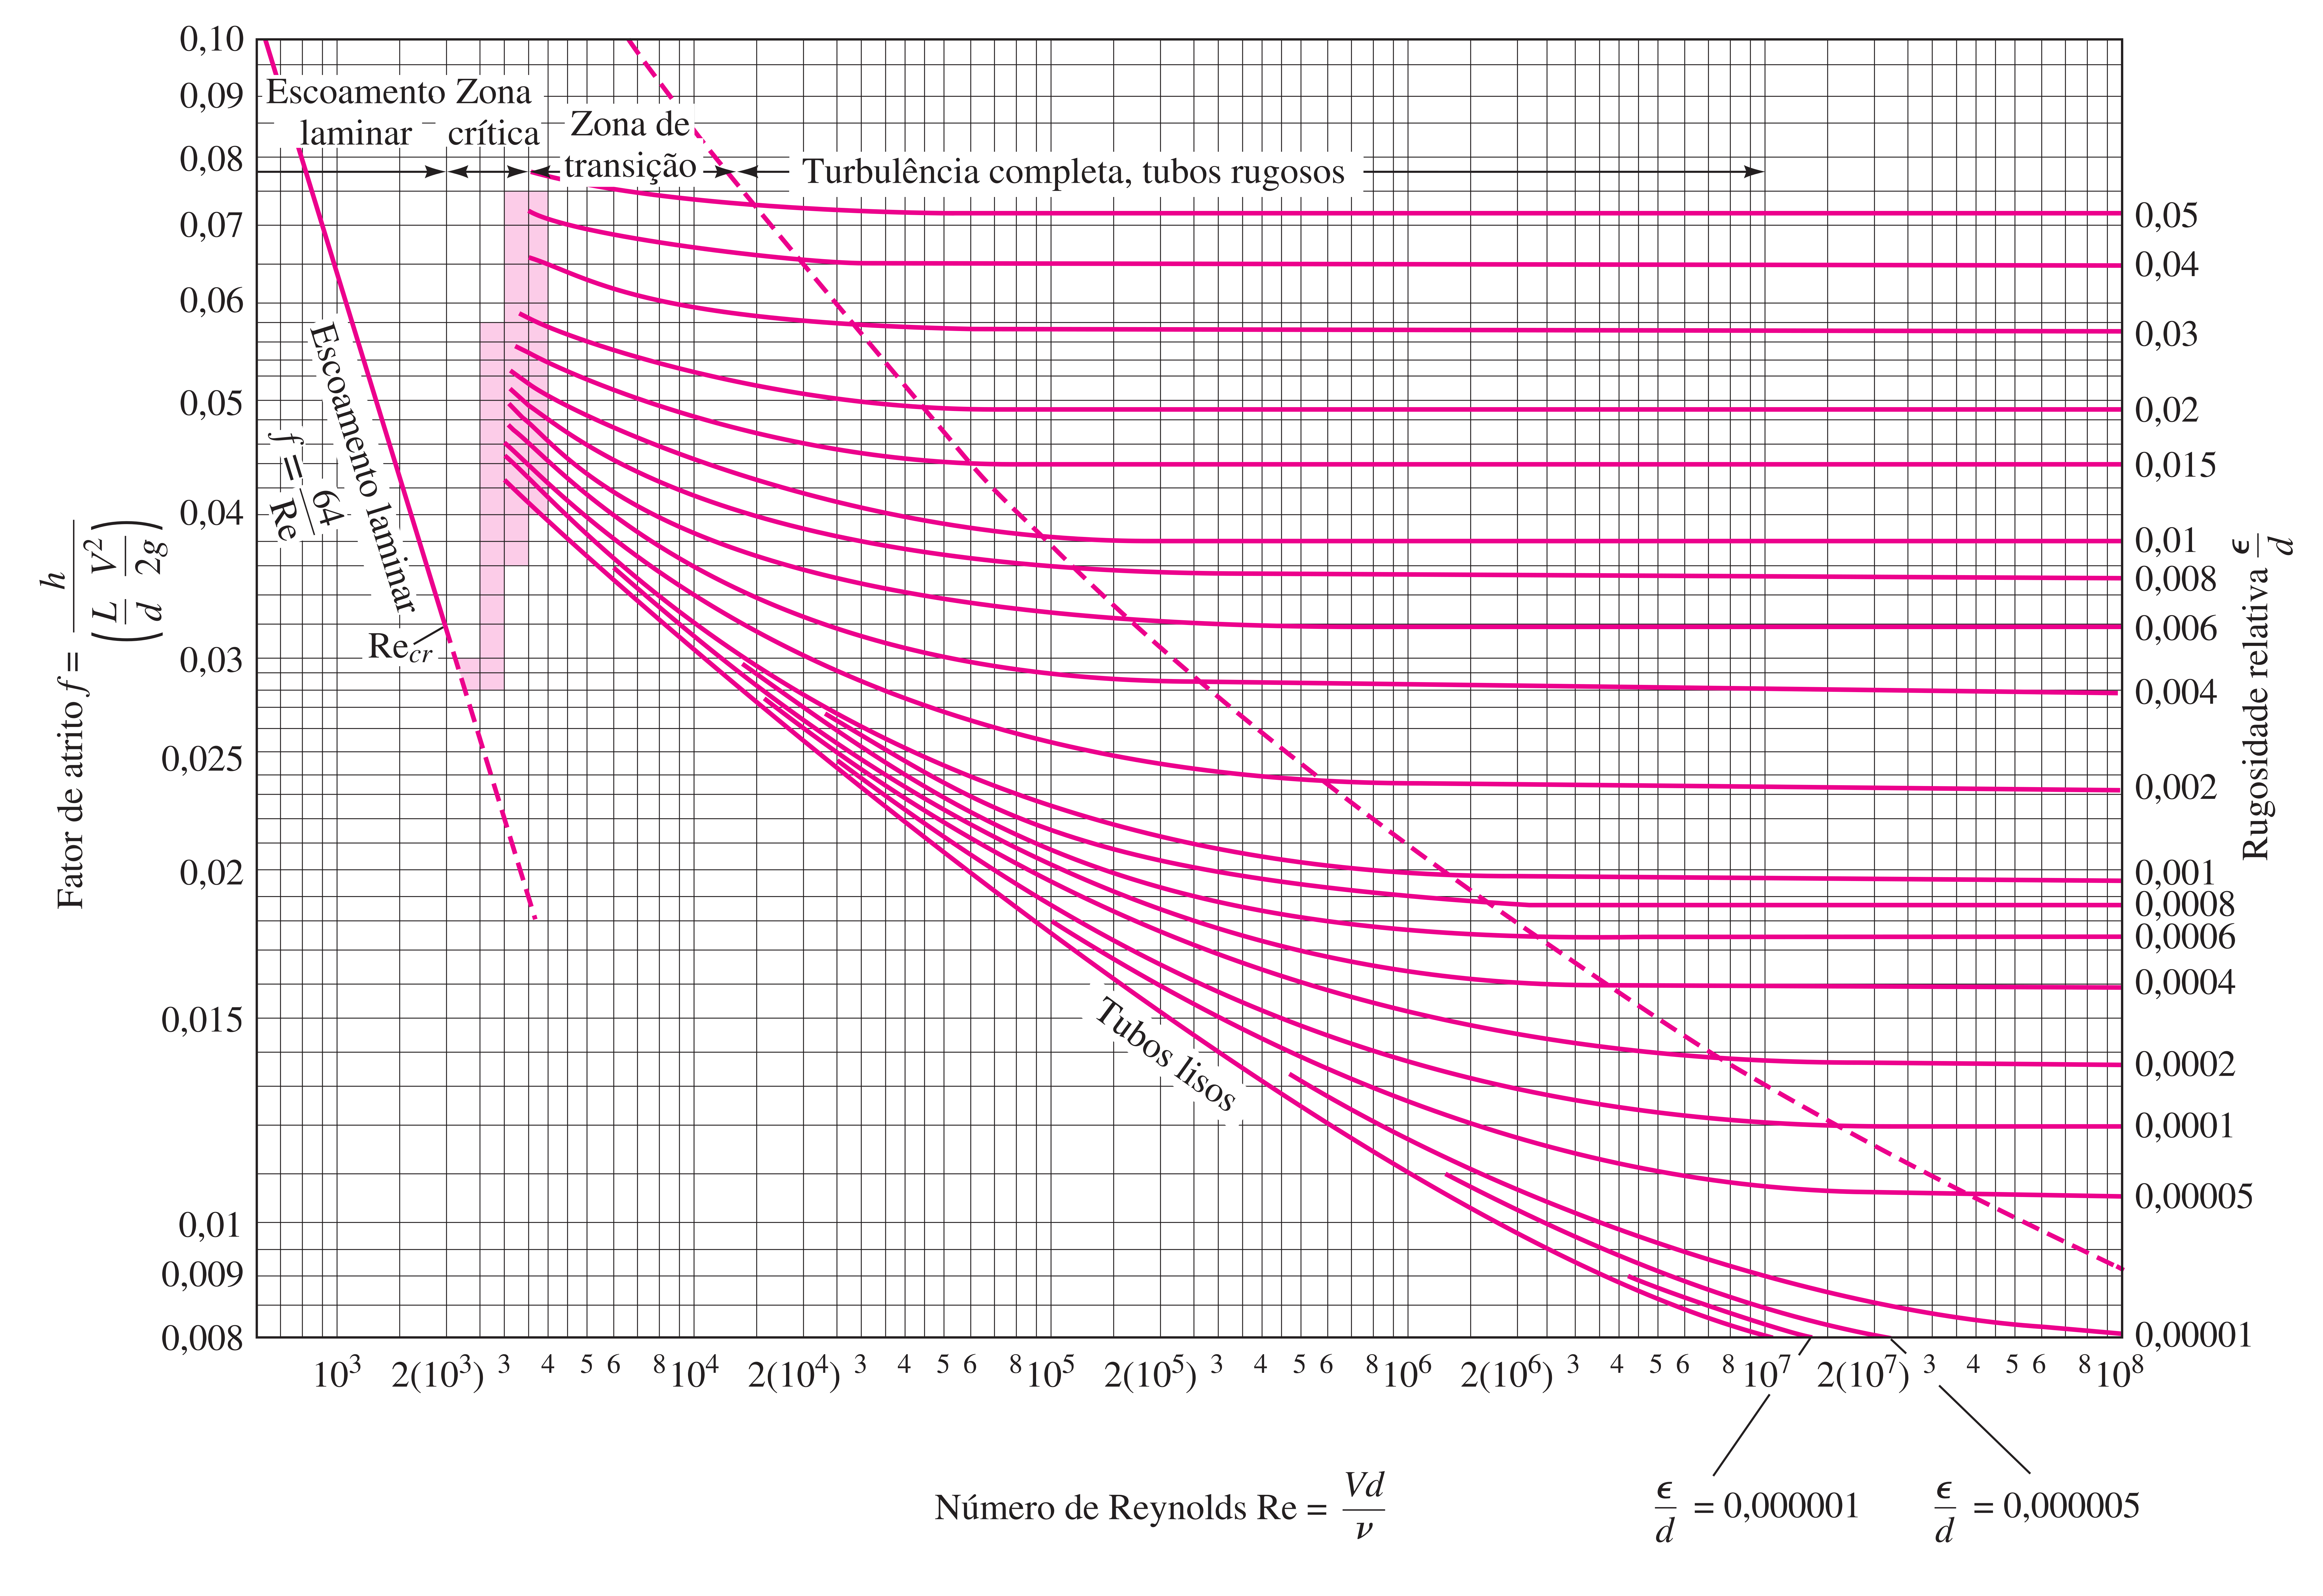
\includegraphics[width=\textwidth]{images/moody_from_white.png}}
\end{frame}
\begin{frame}{Rugosidades}
    \centering
    \vboxcorr{8pt}{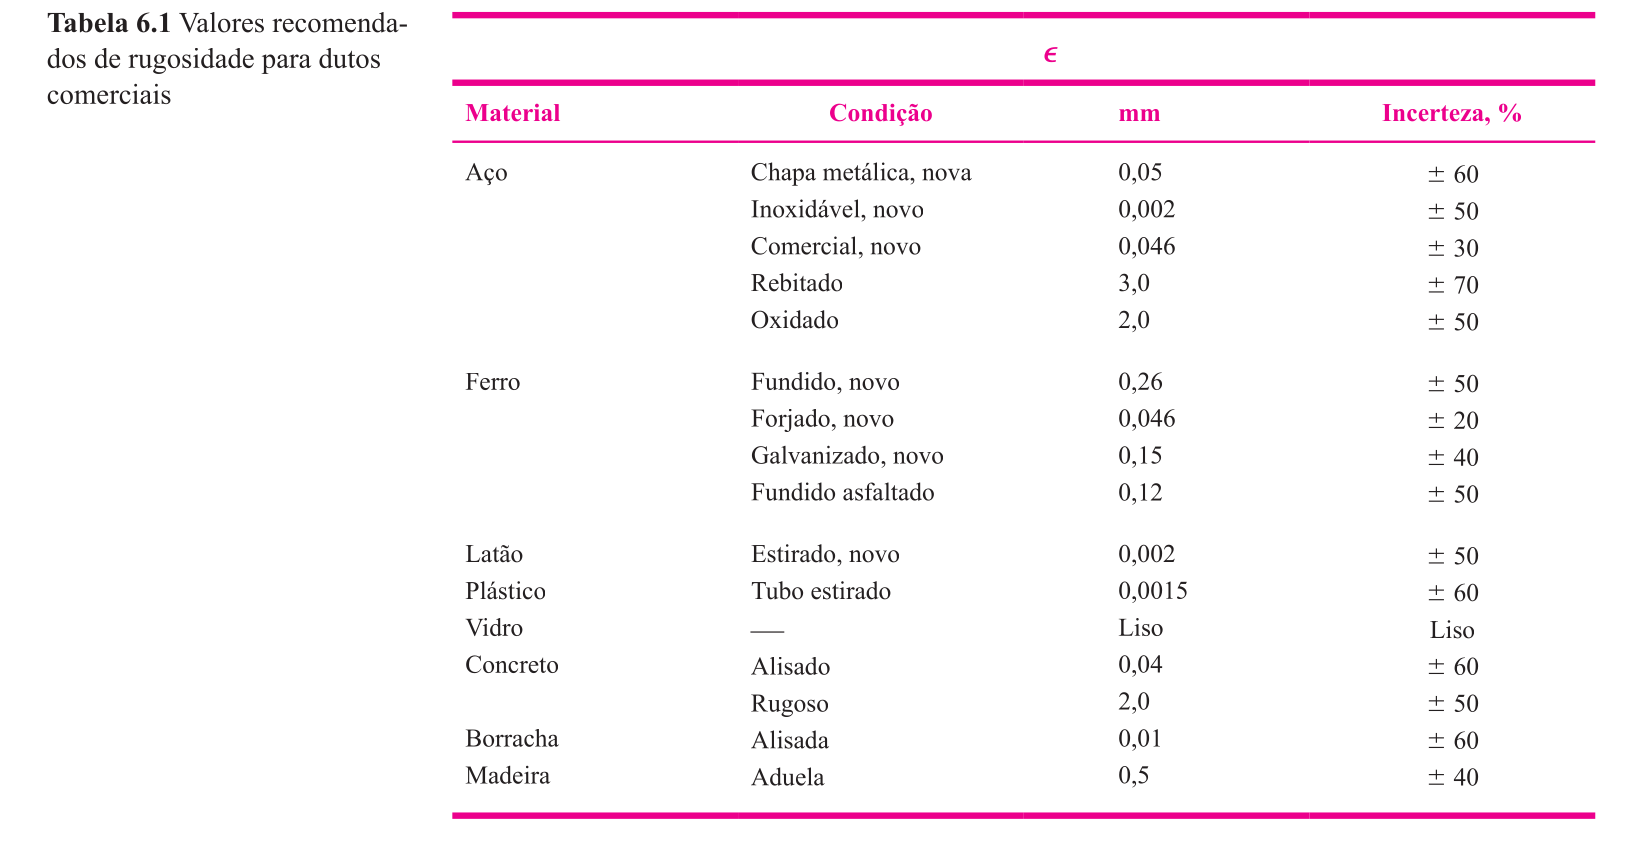
\includegraphics[width=\textwidth]{images/Captura de tela de 2025-05-13 14-11-48.png}}
\end{frame}

\begin{frame}{}
    \begin{itemize} 
        \item Para escoamentos laminares totalmente desenvolvidos em tubulações
            de seção circular, temos que
            \[
                f=\frac{64}{\text{Re}}
            \]
        \item A perda de carga localizada \(h_{pl}\) pode ser obtida por meio da equação
            \[
                h_{pl} = K\frac{V_\text{média}^2}{2g}
            \]
            onde \(K\) é o coeficiente de perda de carga localizada determinado
            experimentalmente e que pode ser encontrado em tabelas e manuais de 
            hidráulica
    \end{itemize}
\end{frame}

\begin{frame}{Exemplo 5.11}
    \begin{minipage}{\textwidth}
        Determine a perda de carga distribuída em um escoamento de água
        (viscosidade \(\mu = \SI{0.001}{Pa\cdot s}\) e massa específica 
        \(\rho = \SI{1000}{kg/m^3}\)) com vazão \(Q= \SI{0.02}{m^3/s}\) num duto,
        com parede de ferro fundido, de seção circular com diâmetro \(D= \SI{10}{cm}\)
        e comprimento \(L=\SI{300}{m}\)
    \end{minipage}

    \vspace{1cm}
    Observação: Segundo o livro, a rugosidade do ferro fundido é \SI{0.24}{mm}
\end{frame}


\begin{frame}{Equação de Colebrook}
    \begin{itemize}
        \item Os valores de \(f\) no diagrama de Moody para escoamentos
            turbulentos\footnote{Para escoamentos laminares vimos que
            \(f=64/\text{Re}\)} \textit{são obtidos} através da \textbf{equação
            de Colebrook}
            \[
                \frac{1}{\sqrt{f}}=
                -\num{2.0}\log_{10} \left(\frac{e/D}{\num{3.7}}+\frac{\num{2.51}}{\text{Re}\sqrt{f}}\right)
            \]
        \item Por exemplo, podemos determinar \(f\) para \(e = \SI{0.24}{mm}\),
            \(D=\SI{10}{cm}\) e \(\text{Re}=\num{2.5e5}\) usando a biblioteca \textit{scipy} no
            \textit{Python}
    \end{itemize}
    \centering
    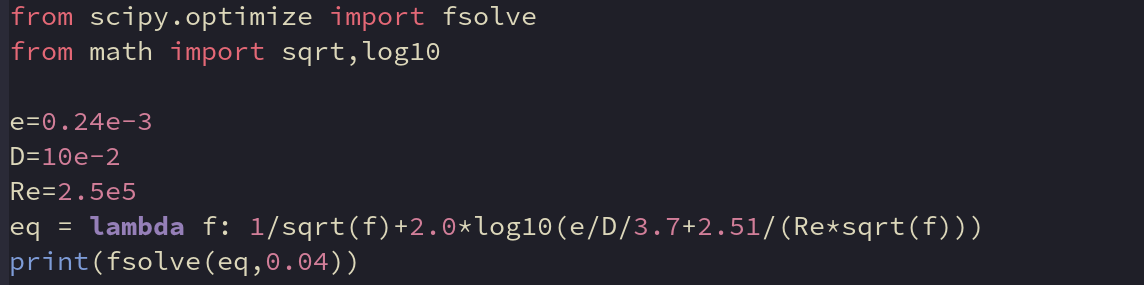
\includegraphics[width=\textwidth]{images/Captura de tela de 2025-05-13 14-30-50.png}
\end{frame}

\begin{frame}{Diagrama de Moody ou equação de Colebrook?}
    \begin{itemize}
        \item Se o problema envolve determinar a perda de carga \(h_{pd}\) ou o comprimento do tubo
            \(L\), o diagrama de Moody é mais adequado pois basta achar o valor de \(f\) através dos valores
            de \(e\), \(D\) e \(\text{Re}\) dados e usar a fórmula de Darcy-Weisbach
            \[
                h_{pd} = f\frac{L}{D}\frac{V_\text{média}^2}{2g}
            \]
        \item Já problemas onde se procura o valor da velocidade de escoamento \(V\) ou o diâmetro do tubo \(D\), o diagrama de Moody
            não é adequado porque não sabemos \(D\) e/ou Re
            \[
                \text{Re} = \frac{\rho V D}{\mu}
            \]

    \end{itemize}
\end{frame}

\begin{frame}{Problemas do livro do White}
    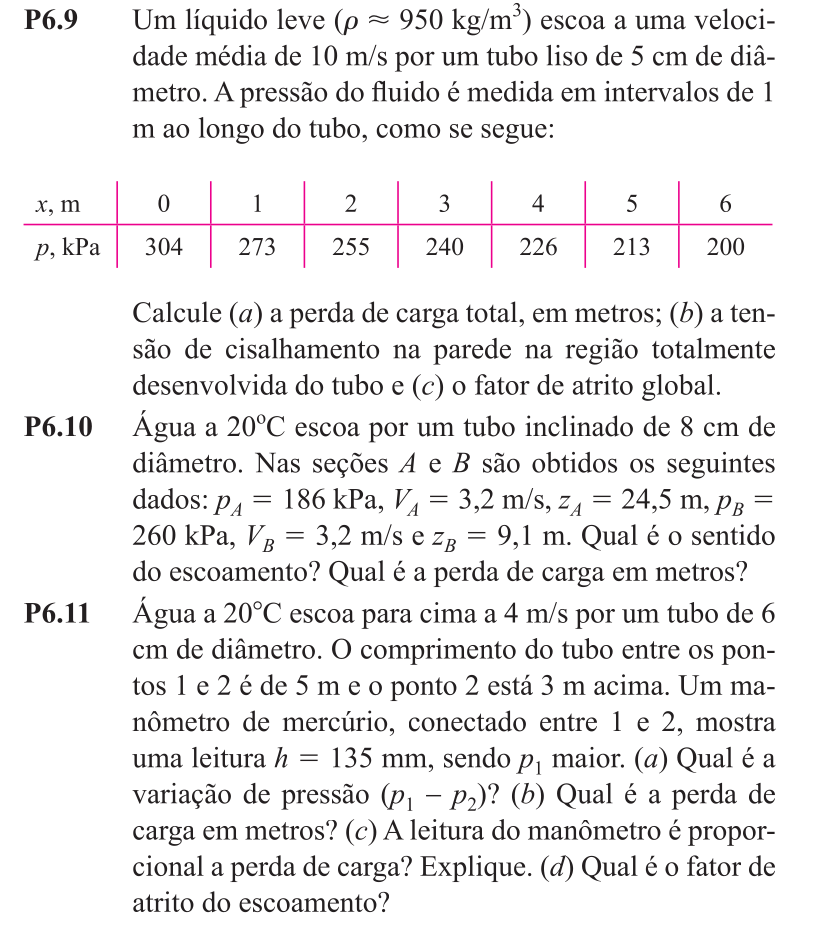
\includegraphics[height=\textheight-28pt]{images/Captura de tela de 2025-05-13 15-07-43.png}
\end{frame}

% \begin{frame}{Problemas do livro do White}
%     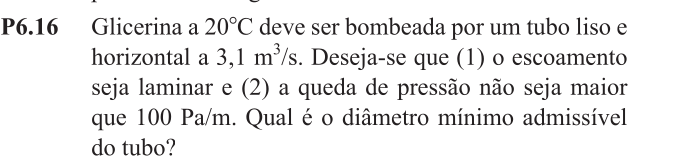
\includegraphics[width=0.5\textwidth]{images/Captura de tela de 2025-05-13 17-16-19.png}
% \end{frame}

\begin{frame}{Problemas do livro do White}
    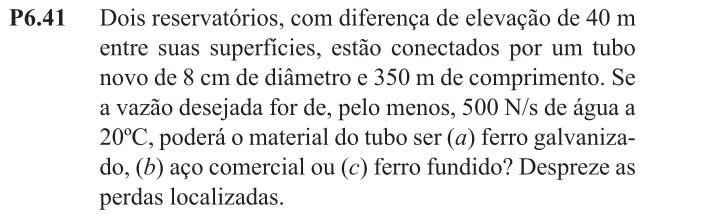
\includegraphics[width=0.5\textwidth]{images/Captura de tela de 2025-05-13 17-30-22.png}
\end{frame}

\begin{frame}{Problemas do livro do White}
    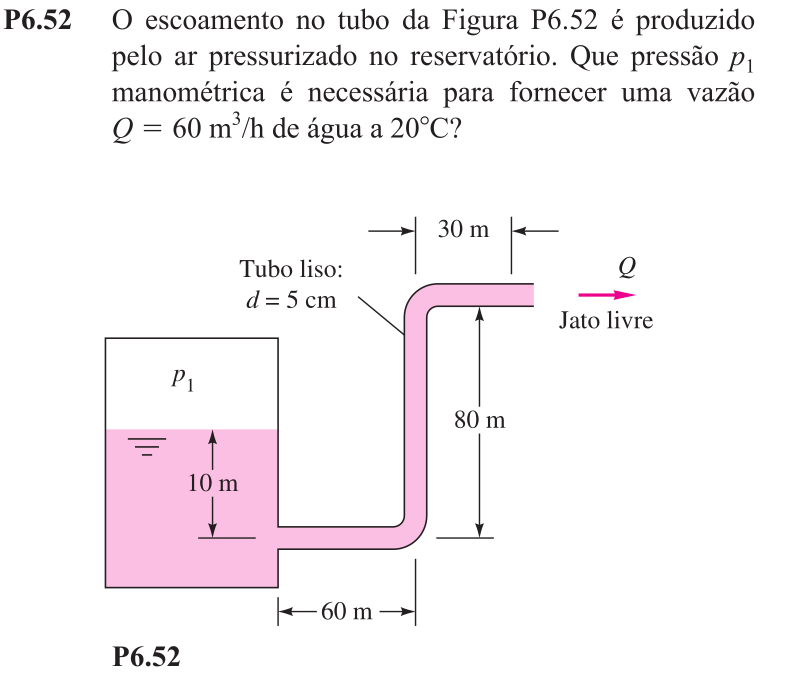
\includegraphics[height=\textheight-28pt]{images/Captura de tela de 2025-05-13 16-56-17.png}
\end{frame}

\begin{frame}{Problemas do livro do White}
    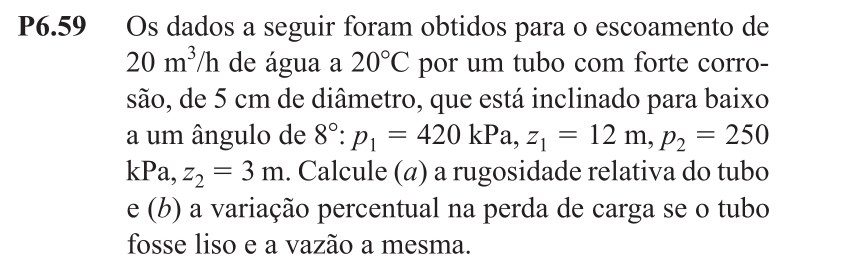
\includegraphics[width=0.5\textwidth]{images/p59.png}

    \includegraphics[width=0.5\textwidth]{images/Captura de tela de 2025-05-13 16-07-08.png}
\end{frame}

\begin{frame}{Problemas do livro do White}
    \includegraphics[width=0.5\textwidth]{images/Captura de tela de 2025-05-13 17-02-19.png}

    \vspace{\fill}
    \tiny{\textit{Observação: Tem cálculo numérico}}
\end{frame}


\begin{frame}{Fim do assunto para a 2\esima{} prova}
    Lista de exercícios:
    \begin{itemize}
        \item Problemas 5.4, 5.5, 5.6, 5.7 e 5.8 do livro texto (Celso Livi)
        \item Problemas 3.1, 3.2, 3.7 e 3.10  do livro auxiliar (Franco Brunneti)
        \item Problemas 6.9, 6.10, 6.11, 6.41, 6.52, 6.59 e 6.61 do livro auxiliar (Frank White)
    \end{itemize}

    A prova terá entre 3 e 4 problemas da lista com \textit{valores numéricos modificados}
\end{frame}

\begin{frame}{Transferência de calor}
    \begin{itemize}
        \item \textbf{Calor} é energia transferida em função de uma diferença de
            temperatura \footnote{Não se pode ter ou armazenar calor}
        \item Existem três mecanismos de transferência de calor: condução, convecção e radiação
        \item A \textbf{condução} ocorre através de um material sólido ou fluido, sem movimento macroscópico da matéria
        \item A \textbf{convecção} ocorre através de um fluido em movimento, com movimento macroscópico da matéria
        \item A \textbf{radiação} ocorre através de ondas eletromagnéticas, principalmente na faixa de infravermelho,
            sem necessidade de meio material
            \pause 
        \item \textbf{Fluxo de calor} é a quantidade de calor que é transferida através de uma superfície por unidade de tempo
        \item \textbf{Densidade de fluxo de calor} é a taxa de transferência de calor por unidade de área
    \end{itemize}
\end{frame}

\begin{frame}{Condução}
    \begin{itemize}
        \item Verifica-se, \textbf{experimentalmente}, que a densidade de fluxo
            de calor \(\vec{q}\) por condução é diretamente proporcional ao gradiente de
            temperatura
            \[
                \vec{q} = -k \nabla T
            \]
        \item Para um processo unidimensional, temos que
            \[
                q_x = -k \frac{dT}{dx}
            \]

    \end{itemize}
\end{frame}

\begin{frame}{Condução unidimensional de calor através de parede de uma camada}
    \begin{itemize}
        \item Seja uma parede plana, de espessura \(L\) e constituída de um
            material com condutividade térmica \(k\) constante
            \begin{center}
                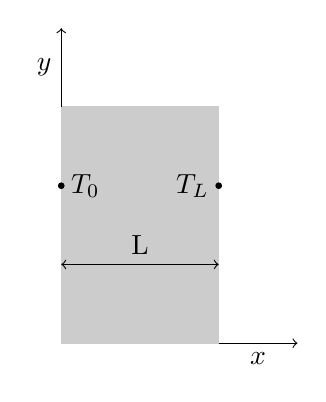
\begin{tikzpicture}
                    \filldraw [black!20] (0,0) rectangle (2,3);
                    \draw [<->] (0,1) -- (2,1) node [midway, above] {L};
                    \filldraw (0,2) circle (1pt) node[right] {$T_0$};
                    \filldraw (2,2) circle (1pt) node[left] {$T_L$};
                    \draw [->] (0,3) -- (0,4) node [midway, left] {$y$};
                    \draw [->] (2,0) -- (3,0) node [midway, below] {$x$};
                \end{tikzpicture}
            \end{center}
        \item As superfícies da parede são mantidas às temperaturas \(T_0\) e
            \(T_L\), constantes, sendo \(T_0 > T_L\)
    \end{itemize}
\end{frame}

\begin{frame}
    \begin{itemize}
        \item Temos que 
            \[
                q_x = -k \frac{dT}{dx} \implies \frac{1}{A}\frac{dQ}{dt}=-k \frac{dT}{dx}
            \]
        \item Considerando um \textit{regime permanente}, temos que a quantidade de calor
            que atravessa a parede por unidade de tempo é constante 
            \[
                \frac{1}{A}\dot{Q_x}=-k \frac{dT}{dx} \implies
                T(x) = T_0 - \frac{\dot{Q_x}}{kA} x
            \]
        \item Ou seja, temos uma distribuição linear de temperatura na parede
    \end{itemize}
\end{frame}

\begin{frame}{Problemas\footnote{Não considerar os trechos marcados em vermelho}}
    \centering
    \begin{tikzpicture}
        \node [inner sep=0] (A) {
            \vboxcorr{74pt}{\includegraphics[width=\textwidth]{images/Captura de tela de 2025-05-27 15-48-58.png}}
        };

        \coordinate (X0) at ($(A.south west)!0.03!(A.south east)$);
        \coordinate (X1) at ($(A.south west)!0.36!(A.south east)$);
        \coordinate (Y0) at ($(A.north west)!0.26!(A.south west)$);
        \coordinate (Y1) at ($(A.north west)!0.29!(A.south west)$);
        \filldraw [red,opacity=0.5] (X0|-Y0) rectangle (X1|-Y1);

        \coordinate (X0) at ($(A.south west)!0.53!(A.south east)$);
        \coordinate (X1) at ($(A.south west)!0.96!(A.south east)$);
        \coordinate (Y0) at ($(A.north west)!0.17!(A.south west)$);
        \coordinate (Y1) at ($(A.north west)!0.20!(A.south west)$);
        \filldraw [red,opacity=0.5] (X0|-Y0) rectangle (X1|-Y1);

        \coordinate (X0) at ($(A.south west)!0.50!(A.south east)$);
        \coordinate (X1) at ($(A.south west)!0.58!(A.south east)$);
        \coordinate (Y0) at ($(A.north west)!0.20!(A.south west)$);
        \coordinate (Y1) at ($(A.north west)!0.23!(A.south west)$);
        \filldraw [red,opacity=0.5] (X0|-Y0) rectangle (X1|-Y1);
    \end{tikzpicture}
\end{frame}


\begin{frame}{Condução unidimensional de calor através de parede cilíndrica}
    \begin{itemize}
        \item Seja um duto cilíndrico longo, de comprimento \(L\), com raio interno \(r_i\) e
            raio externo \(r_e\) construído de um material com condutividade térmica \(k\) constante
        \item As superfícies interna e externa do duto são mantidas às temperaturas \(T_i\) e \(T_e\),
            respectivamente, constantes, sendo \(T_i > T_e\)
            \begin{center}
                \vboxcorr{152pt}{\includegraphics[height=\textheight]{images/Captura de tela de 2025-05-27 16-04-45.png}}
            \end{center}
        \item Considerando que a condução de calor é unidimensional na direção radial e em regime permanente,
            \textit{facilmente} encontramos que
            \[
                T(r) = T_i - \frac{\dot{Q_r}}{2\pi k L} \ln\left(\frac{r}{r_i}\right)
            \]

    \end{itemize}
\end{frame}

\begin{frame}{Problemas}
    \begin{columns}[T]
        \begin{column}{0.45\textwidth}
            \vboxcorr{57pt}{\includegraphics[width=\textwidth]{images/Captura de tela de 2025-05-27 16-28-16.png}}
        \end{column}
%%%%%%%%%%%%%%%%%%%%%%%%%%%%%%%%%%%%%%%%%%%%%%%%%%
        \begin{column}{0.45\textwidth}
            \hboxcorr{20pt}{\includegraphics[width=\textwidth]{images/Captura de tela de 2025-05-27 16-29-31.png}}
        \end{column}
    \end{columns}
\end{frame}

\begin{frame}{Resistência térmica}
    \begin{itemize}
        \item \textit{Sabemos que} corrente elétrica num fio condutor \(I\) é a quantidade de carga 
            elétrica que passa pela área da seção reta por unidade de tempo
            \[
                I = \frac{d\color{red}Q}{dt}
            \]
        \item \textit{Sabemos que} fluxo de calor \(\dot{Q}\) é a quantidade de calor que atravessa
            uma superfície por unidade de tempo
        \item \textit{Da mesma forma} que temos resistência elétrica podemos ''ter'' 
            resistência térmica onde
            \[
                \dot{\color{blue}Q} = \frac{\Delta T}{\sum R_T}
            \]
        \item Definimos as resistências térmicas de uma parede plana com \textbf{convecção} no
            contorno
            \[
                R_{T,\text{convecção}} = \frac{1}{hA} \quad \quad
                R_{T,\text{condução}} = \frac{L}{kA}
            \]
            onde \(L\) é a espessura da parede, \(k\) é a condutividade térmica e
            \(h\) é o coeficiente de transferência de calor por convecção
    \end{itemize}
\end{frame}

\begin{frame}[c]
    \begin{itemize}
        \item De forma análoga ao modelo elétrico, temos que resistências em
            série se somam para dar a resistência equivalente e em paralelo
            temos que a resistência equivalente é o recíproco da soma dos
            recíprocos das resistências
    \end{itemize}
\end{frame}

\begin{frame}{Problemas}
    \centering
    \vboxcorr{147pt}{
        \shortstack{%
            \includegraphics[width=\textwidth]{images/Captura de tela de 2025-06-24 15-13-40.png}\\%
            \includegraphics[width=\textwidth]{images/Captura de tela de 2025-06-24 15-13-57.png}%
            }
        }
\end{frame}

\begin{frame}{Problemas}
    \centering
    \includegraphics[height=\textheight-28pt]{images/Captura de tela de 2025-06-24 15-40-03.png}
\end{frame}

\begin{frame}{Problemas}
    \centering
    \includegraphics[height=\textheight-28pt]{images/Captura de tela de 2025-06-24 15-43-56.png}
\end{frame}

\begin{frame}[c]{Resistência térmica para uma parede cilíndrica}
    Temos que
    \[
        R_{T,\text{convecção}} = \frac{1}{2\pi r L h} \quad \quad
        R_{T,\text{condução}} = \frac{1}{2\pi L k}\ln\left(\frac{r_e}{r_i}\right)
    \]
\end{frame}

\begin{frame}{Problemas 8.8 e 8.9}
    \centering
    \includegraphics[height=\textheight-28pt]{images/Captura de tela de 2025-06-24 16-45-05.png}
\end{frame}

\begin{frame}{Fim do assunto para a 3\esima{} prova}
    Lista de exercícios:
    \begin{itemize}
        \item Problemas 8.1, 8.2, 8.3, 8.4, 8.5, 8.6, 8.7, 8.8, 8.9, 8.12, 8.13, 8.14, 8.15 e 8.16 do livro texto (Celso Livi)
    \end{itemize}

    A prova terá entre 3 e 4 problemas da lista com \textit{valores numéricos modificados}
\end{frame}

\end{document}
